%*********************************************************************
% 中国人民大学硕士毕业论文模板
% Copyright 2022 Ruoyang Guo, Pan Du
% 2020/06/06 v1.0 beta
%
%本文编写的依据是中国人民大学教务处2018年修订的《研究生毕业论文（设计）指导手册》
%本文的给出例子是在Qiu Renxiang本科毕业论文，Pan Du 硕士论文模版上进行改造。
%本文基本满足手册中对硕士论文的格式要求，并自动生成图表目录并编号，引用和目录也都具有超链接
% 重要提示：
%   1. 请确保使用 UTF-8 编码保存
%   2. 请使用 XeLaTeX编译
%   3. 修改、使用、发布本文档请务必遵循 LaTeX Project Public License
%   4. 不需要的注释可以尽情删除
%*********************************************************************
\documentclass[12pt,UTF8,twoside]{ctexart}

\usepackage{amsthm}
\newtheoremstyle{mystyle}{}{}{\upshape}{}{\bfseries}{:}{.5em}{}
\theoremstyle{mystyle}
\newtheorem{theorem}{定理}
\newtheorem{definition}{定义}
\newtheorem{property}{性质}
\newtheorem{lemma}{引理}


\usepackage{amsmath,amssymb,amsfonts}
\usepackage{algpseudocode}
\usepackage{float}
\usepackage[super]{cite}  % 上标引用格式
\usepackage{listings}
\usepackage{graphicx}
\usepackage{booktabs}
\usepackage{multirow}
\usepackage{geometry}
\usepackage{appendix}
\usepackage{hyperref}
\usepackage[shortlabels]{enumitem}
\usepackage{threeparttable}
\usepackage{fancyhdr}
\usepackage{setspace}
\usepackage[T1]{fontenc}
%\usepackage{mathptmx}%Times New Roman字体
\usepackage{titletoc}
\usepackage{fontspec}
\usepackage{pdfpages}
\usepackage{tikz}
\usepackage{etoolbox}
\usepackage{xcolor}
\usepackage{caption}
\usepackage{array}
\usepackage{titlesec}
%\usepackage{subfigure}
\usepackage{diagbox}
\usepackage{bbm}
%\usepackage{algorithm}
%\usepackage{algorithmicx}
% \usepackage{algorithmic}
% \usepackage{algorithm2e}
% \usepackage[ruled]{algorithm2e}                                     %算法排版样式1
% \usepackage[ruled,vlined]{algorithm2e}                          %算法排版样式2
% \usepackage[linesnumbered,boxed]{algorithm2e} 


%pam
\usepackage{bm}
\usepackage[ruled,linesnumbered]{algorithm2e}
\usepackage{subfig}
\usepackage{makecell}
\usepackage{bibspacing}
\setlength{\bibspacing}{0\baselineskip}
\setlist[enumerate]{itemsep=0pt,parsep=0pt,topsep=4pt,partopsep=0pt}
\setlist[itemize]{itemsep=0pt,parsep=0pt,topsep=4pt,partopsep=0pt}

\usepackage{afterpage}
\newcommand\myemptypage{
    \null
    \thispagestyle{empty}
    \addtocounter{page}{-1}
    \newpage
    }
    
\newcommand{\eref}[1]{(\ref{#1})}
%pam


%图表目录重定义
%\renewcommand {\thetable} {\thesection{}.\arabic{table}}
%\renewcommand {\thefigure} {\thesection{}.\arabic{figure}}

\renewcommand {\thetable} {\thesection{}-\arabic{table}}
\renewcommand {\thefigure} {\thesection{}-\arabic{figure}}
\makeatletter
\@addtoreset{figure}{section}
\@addtoreset{table}{section}
\makeatother
\DeclareCaptionLabelSeparator{twospace}{\ ~}  
\captionsetup{labelsep=twospace}


\renewcommand{\algorithmicrequire}{\textbf{输入:}}  
\renewcommand{\algorithmicensure}{\textbf{输出:}}  
\floatname{algorithm}{算法}


\renewcommand{\KwIn}{\textbf{输入:}}  
\renewcommand{\KwOut}{\textbf{输出:}}  
\renewcommand{\algorithmcfname}{算法}

%博士学生毕业论文要求纵向打印，页边距的要求为：
%上（T）：45mm
%下（B）：40mm
% 左（L）：35mm
% 右（R）：30mm
% 装订线（T）：0.5 cm
% 装订线位置（T）：左

\geometry{a4paper,left = 3.5cm,right = 3cm,top = 4.5cm,bottom= 4cm}
\setlength{\headheight}{15pt}


% 页眉：学校标志（教务处主页提供下载）：
% 高度为0.98 cm，宽度为4.13 cm，居中放置。
% 页码采用10.5号宋体字，居中放置，格式为：第1页。

\pagestyle{empty}
\lhead{}
\chead{}
\rhead{}
\lfoot{}
\rfoot{}

%目录和引用超链接
\hypersetup{
colorlinks=true,
linkcolor=black,
citecolor=black
}

\begin{document}
\hypersetup{pageanchor=false}

\newcommand\dunderline[3][-1pt]{{%
  \setbox0=\hbox{#3}
  \ooalign{\copy0\cr\rule[\dimexpr#1-#2\relax]{\wd0}{#2}}}}

%添加封面
\begin{titlepage}
  \vspace*{-10mm}
  \centering

  
\includegraphics[scale = 1.5]{Cover_figure/title.jpg}

  \vspace*{3mm}

  \zihao{1}\heiti 硕士学位论文

  \vspace*{3mm}
  \zihao{5}\heiti THESIS OF MASTER DEGREE
  \vspace{20mm}

  % ================= 题目区 =================
  \flushleft
  \begin{spacing}{1.5}

    % 论文题目（中文）第一行
    \centering\heiti\Large\selectfont{%
      论文题目：\dunderline[-3pt]{0.8pt}{\makebox[110mm][c]{基于数据感知的多智能体专利分析}}}

    % 论文题目（中文）第二行
    \centering\heiti\Large\selectfont{%
      \phantom{论文题目：}\dunderline[-3pt]{0.8pt}{\makebox[110mm][c]{系统设计与实现}}}

    \vspace{2mm}

    % 论文题目（英文）第一行
    \centering\heiti\Large\selectfont{%
      （英\hspace{7mm}文）：\dunderline[-3pt]{0.8pt}{\makebox[110mm][c]{Design and Implementation of Data-Aware}}}

    % 论文题目（英文）第二行
    \centering\heiti\Large\selectfont{%
      \phantom{（英\hspace{7mm}文）：}\dunderline[-3pt]{0.8pt}{\makebox[110mm][c]{Multi-Agent Patent Analysis System}}}

    \vspace{6mm}

    \centering\heiti\Large\selectfont{作\hspace{12mm}者：\dunderline[-3pt]{0.8pt}{\makebox[110mm][c]{于鹏鹏}}}

    \centering\heiti\Large\selectfont{指导教师：\dunderline[-3pt]{0.8pt}{\makebox[110mm][c]{黄科满}}}

    \centering\heiti\Large\selectfont{完成日期：\dunderline[-3pt]{0.8pt}{\makebox[110mm][c]{2026年3月}}}
  \end{spacing}

  \vfill

\end{titlepage}


%%添加摘要
\newpage
\section*{摘\ \ 要}

针对专利计量研究中”分析方案依赖人工设计、自动化系统规划能力不足”的问题，本文提出一种数据感知驱动的多智能体专利分析框架。现有大语言模型系统在代码执行与报告生成方面已具备一定能力，但在方案设计阶段普遍缺少对真实数据分布与结构特征的前置感知，导致任务容易模板化、结论针对性不足。为解决该问题，本文构建了由规划智能体、方法规格化智能体、执行智能体和评审智能体组成的四智能体协作系统，并通过工作流编排框架实现端到端流程管理。

在方法上，本文提出三项关键机制。第一，数据感知前置机制：在规划前引入数据预览与图结构预览模块，提取列级统计、跨列关系、图结构特征和分层抽样语义样本，并驱动大语言模型生成可检验研究洞察。第二，双知识图谱协同机制：将因果图谱用于约束研究假设空间，将方法图谱用于约束分析执行空间，实现”理论解释”与”方法可执行”的协同。第三，两轮迭代优化机制：以第一轮执行结果为反馈，触发第二轮差距修补与验证性分析，形成”探索—验证”闭环。

实验采用四方案渐进叠加与两组组件消融设计，在三个典型专利计量问题上对 6 种模式各重复运行 5 次，共完成 90 组实验。结果表明，完整方案（C\_iterative）在四方案主实验与六模式总览中均保持最高平均总分（23.87/25），且在相关性、针对性、方法合理性、创新性和深度五个维度上表现最稳定。相比 A\_template 与 D\_baseline0，B\_data\_aware 在重复实验中稳定取得更高语义评分和更强的数据证据引用，说明数据感知是推动方案从“问题语义驱动”转向“数据证据驱动”的关键环节。组件消融结果进一步表明，移除数据感知或知识图谱都会降低平均表现，其中数据感知对针对性引用和方案聚焦的贡献更直接；知识图谱收益则具有任务依赖性，在结构锚点清晰、分析链条较长的问题上作用更明显，而在开放度更高的问题上需要避免静态路径过度约束。

本文工作从”执行自动化”进一步推进到”规划自动化”，为专利计量分析提供了可复现、可追踪的系统化实现方案，并在所测试的三个研究问题上展示出初步工程可行性，对技术情报分析和知识产权决策具有参考价值。

\vspace{1em}
\noindent\textbf{关键词：}多智能体系统；专利计量；数据感知；知识图谱；自动化分析

\newpage
\section*{Abstract}

This thesis addresses a core limitation in patent analytics automation: existing LLM-based systems are increasingly capable at execution but still weak at analysis planning. In many cases, plans are generated without sufficient grounding in dataset-specific evidence, resulting in template-like tasks and limited specificity. To solve this problem, we design a data-aware multi-agent framework for patent analytics, including four specialized agents (planning agent, specification agent, execution agent, and review agent), orchestrated by a workflow management framework.

The proposed method contains three key components. First, a pre-planning data-awareness mechanism introduces DataPreview and GraphPreview to extract column-level statistics, cross-column relations, graph-structural signals, and stratified semantic samples, then converts them into testable insights through LLM reasoning. Second, a dual-knowledge-graph collaboration mechanism is designed: a causal graph constrains hypothesis space, while a method graph constrains executable analysis space. Third, a two-round iterative mechanism refines plans using first-round execution feedback, enabling an exploration-to-validation loop.

We evaluate the framework with progressive accumulation across four modes (D\_baseline0, A\_template, B\_data\_aware, C\_iterative) and two component ablation settings on three representative patent bibliometrics tasks. Each of the six modes is repeated five times, yielding 90 runs in total. Across repeated experiments, C\_iterative achieves the highest overall average score (23.87/25) and remains the most stable top-performing configuration. Compared with A\_template and D\_baseline0, B\_data\_aware consistently improves semantic quality and evidence grounding, indicating that data awareness is the main driver that shifts planning from question-driven generation toward evidence-driven generation. Ablation results further show that removing either data awareness or knowledge graphs lowers the average performance; however, the gain from knowledge-graph guidance is task-dependent, helping more on problems with clear structural anchors and multi-step analytic chains than on more open-ended tasks.

The study advances automation from execution-level to planning-level intelligence and provides a reproducible, extensible, and traceable framework for real-world patent analytics, with preliminary engineering feasibility demonstrated on the three tested questions.

\vspace{1em}
\noindent\textbf{Keywords: }multi-agent system; patent bibliometrics; data awareness; knowledge graph; automated analytics


% \myemptypage

%%添加目录
\newpage
\hypersetup{pageanchor=false}
\setcounter{page}{1}
\pagenumbering{arabic}
\pagestyle{fancy}
% \pagestyle{empty}
\lhead{}
\chead{}
\rhead{}
\lfoot{}
\rfoot{}
\fancyfoot[C]{\footnotesize \thepage}
\setlength{\topskip}{0pt}
\renewcommand\contentsname{目\ 录}
\renewcommand\listfigurename{图\ 目\ 录}
\renewcommand\listtablename{表\ 目\ 录}
\tableofcontents
\newpage
\listoffigures
\listoftables
\newpage

% \myemptypage


% \fancyfoot[C]{\songti 第\thepage 页}
\hypersetup{pageanchor=true}
\setcounter{page}{1}
\pagenumbering{arabic}
\pagestyle{fancy}
\renewcommand{\headrulewidth}{.5pt}
\lhead{}
\chead{基于数据感知的多智能体专利分析系统设计与实现}
\rhead{}
\lfoot{}
\rfoot{}
\fancyfoot[C]{\footnotesize \thepage}
% \rfoot{\footnotesize \thepage }
% 按照自然段依次排列，每段起行空两格，回行顶格。12号宋体字，（重点文句，12号宋体字，加粗），倍行距20pt。
%正文、注释双面打印，编排页码，自第1页起，设置页眉。
%大标题(第1章)       黑体小二号（18pt），占六行（按宋体小四号计）居中
\titleformat{\section}[block]{\centering\heiti\LARGE}{第\arabic{section}章}{1em}{}[]
\titlespacing{\section}{0pt}{27pt}{27pt}
%一级节标题（1.1）    黑体小三号（14pt），占四行（按宋体小四号计）顶头
\titleformat{\subsection}[block]{\heiti\Large}{\arabic{section}.\arabic{subsection}}{1em}{}[]
\titlespacing{\subsection}{0pt}{17pt}{17pt}
%二级节标题（1.1.1）  黑体小四号（12pt），占两行（按宋体小四号计）顶头
\titleformat{\subsubsection}[block]{\heiti\large}{\arabic{section}.\arabic{subsection}.\arabic{subsubsection}}{1em}{}[]
\titlespacing{\subsubsection}{0pt}{6pt}{6pt}
%倍间距20pt
\setlength{\baselineskip}{20pt}


\newpage
\setcounter{table}{0}
\setcounter{figure}{0}
\section{绪论}

\subsection{研究背景与意义}

专利文献及其结构化元数据是技术创新活动的重要外显载体。与普通科技文本相比，专利数据同时具有"技术属性、法律属性、时间属性、组织属性"四重特征，这使其天然适合用于技术演化分析、竞争态势分析和创新能力评估\cite{basberg1987patents,trajtenberg1990penny,daim2006forecasting}。长期以来，专利计量分析在科技政策制定、企业技术战略规划和创新能力评估中发挥着不可替代的作用\cite{griliches1990patent,narin1997increasing,zhu2014patent}。专利引用数据作为知识流动的重要指标，已被广泛用于测度技术影响力和知识溢出效应\cite{hall2001nber,jaffe2000knowledge}。

然而，在实际研究场景中，专利计量分析仍高度依赖人工流程：研究者通常需要手工定义变量、挑选统计方法、设置控制变量并反复调整分析路径。该过程的专业门槛高、耗时长、复现实验成本大，且在面对新问题时迁移效率较低\cite{vanzeebroeck2011filing,mejia2024patent}。

近年来，大语言模型（Large Language Model, LLM）推动了自动化数据分析系统的快速发展\cite{zhao2024llm,brown2020language}。已有工作在任务分解、代码生成、执行纠错等方面取得显著进展，例如 DS-Agent\cite{guo2024dsagent}、Data Interpreter\cite{hong2025data} 等系统展示了多智能体协作在复杂分析任务中的可行性。多智能体框架如 AutoGen\cite{wu2023autogen}、MetaGPT\cite{hong2024metagpt} 等进一步提供了可编程的协作机制，使得构建复杂的端到端分析系统成为可能\cite{wang2024survey}。

但现有系统的优化重点主要集中在"执行层"，即如何更稳定地完成既定分析任务；对于"规划层"，即如何在给定研究问题与具体数据集时自动形成高质量分析方案，现有方法仍不充分\cite{sun2025survey}。该问题在专利计量场景中尤为突出，因为专利变量关系复杂、字段语义多样、跨列关联隐含，若缺乏前置数据感知，系统易产生模板化、泛化但不贴合数据事实的方案。

另一方面，知识图谱增强 LLM 已成为热点方向。GraphRAG\cite{edge2024graphrag} 等研究表明，图结构能够提升复杂问题的全局信息组织能力。在知识图谱与 LLM 的融合路线上，已有系统性的路线图综述\cite{pan2024unifying}。在专利领域，EvoPat\cite{wang2024evopat}、KLIPA\cite{deng2025klipa} 等工作开始尝试将 LLM 与知识组织或检索能力结合。

但总体上，已有研究更多服务于问答、摘要、检索等文本任务；针对"专利结构化数据上的分析方案自动设计"仍缺少系统性方法\cite{jiang2025natural}。由此，本文聚焦"数据感知驱动的多智能体专利分析方案生成"，试图补足从执行自动化到规划自动化的关键环节。

从实践价值看，若能在规划前自动提取数据分布、图结构、样本语义等证据信息，并将其与领域知识约束协同使用，可显著降低人工试错成本，提高研究可复现性与结论可解释性。对专利计量研究者、技术情报分析师和企业知识产权部门而言，这一能力均具有直接应用价值。

\subsection{研究问题与研究内容}

围绕上述背景，本文的核心研究问题定义为：如何构建一个面向专利计量分析场景的多智能体系统，使其能够在给定具体专利数据集与研究问题的前提下，自动生成具有数据感知能力的分析方案，并在执行反馈基础上持续迭代优化，从而稳定提升分析结果的针对性、可解释性与整体质量。与仅关注代码生成或单步任务执行的自动化方法不同，本文更关注“分析方案如何被规划出来”这一前置问题，即如何让系统在正式执行之前，先形成与当前数据特征、研究目标和领域知识相匹配的分析思路。

为回答该问题，本文围绕方案生成过程中的“数据依据从何而来”“理论与方法如何约束”“系统如何持续改进”三个关键环节，开展以下三项研究内容：

第一，提出数据感知方案生成机制。系统在正式规划前，并不直接根据自然语言问题生成分析步骤，而是首先通过 DataPreview 提取列级统计、字段类型、缺失情况与跨列关系等信息，通过 GraphPreview 提取专利网络中的结构特征，并结合分层抽样摘要触发 LLM 生成“可检验洞察”。这些洞察并非泛化表述，而是能够被后续统计分析、建模过程或代码执行直接验证的候选判断。该方法的目标，是将“数据事实”显式注入规划上下文，使后续方案生成不再只依赖语言模型对任务表述的语义理解，而是建立在对当前数据集真实结构的感知基础之上，从而减少模板化、空泛化和脱离样本实际的问题。

第二，设计双知识图谱协同机制。本文将因果图谱用于约束“研究假设空间”，将方法图谱用于约束“分析执行空间”，并在规划阶段实现二者联动\cite{pan2024unifying,liu2016knowledge}。其中，因果图谱主要回答“哪些变量关系值得被优先考察、哪些路径具备理论上的可解释性”，方法图谱则进一步回答“这些变量可以如何被测度、这些关系适合采用什么分析方法进行验证”。通过将两类图谱分别作用于假设形成与方法选择两个层面，系统能够在保持一定生成灵活性的同时，避免分析路径完全依赖大模型自由发挥。该机制的核心价值，在于把专利分析中的领域知识、变量结构与方法经验沉淀为可调用、可组合、可约束的图谱资源，从而提升方案的理论一致性与执行可行性。

第三，构建两轮迭代优化机制。第一轮聚焦探索性分析，目标是在数据感知结果与图谱约束的基础上快速形成较为完整的初始分析蓝图，并识别出具有潜在价值的变量关系、比较维度和方法路径；第二轮则基于第一轮执行结果进行差距识别、方案修正和验证性深化，形成“探索—验证”闭环。与一次性输出方案的方式相比，两轮迭代设计能够让系统显式吸收执行阶段暴露出的不足，例如变量选择不充分、方法与数据不匹配、结论支撑证据不足等问题，并据此对后续规划进行补强。该方法有助于提升分析深度、机制解释能力和结论稳健性，使系统输出更接近真实研究过程中的渐进式推理与修正逻辑。

\subsection{研究方法与技术路线}

本文采用“系统构建 + 渐进叠加 + 组件消融 + 重复实验 + 双轨评估”的研究方法。整体上，本文并非仅从算法性能提升的角度展开研究，而是遵循“先构建可运行系统原型，再通过渐进实验和消融实验识别关键模块贡献，最后以多维指标和重复实验验证方法有效性”的技术路线推进。该路线兼顾了系统研究的工程实现要求与学术研究的可解释性要求，能够较为完整地回答“系统是否可实现”“改进是否真实有效”“提升究竟来自何种机制”以及“这些提升是否在重复运行下仍然成立”等核心问题。

在系统构建层面，本文基于工作流编排框架\cite{langgraph2024}设计四智能体协作流程：规划智能体负责分析蓝图生成，方法规格化智能体负责任务技术规格化，执行智能体负责代码生成与纠错执行，评审智能体负责结果校验与报告生成。系统以状态机方式组织任务流，支持结构化输入、过程追踪与结果落盘。在这一基础上，本文进一步将数据预览、图结构预览、双知识图谱调用、任务规格化与结果反馈等能力嵌入统一工作流中，使系统不只是“多代理串联”，而是形成从问题理解、方案规划、代码执行到结果回评的闭环式分析流程。这样的设计有助于提升系统在复杂专利计量任务中的模块协同性、过程透明度与故障可定位性。

在实验层面，本文采用四方案渐进叠加设计：D\_baseline0（纯 LLM）、A\_template（仅知识图谱模板）、B\_data\_aware（知识图谱+数据洞察）、C\_iterative（知识图谱+数据洞察+两轮迭代，完整模式）。该设计遵循“由简到繁、逐层加能”的思想，通过控制变量的方式依次引入知识约束、数据感知和迭代优化机制，使每一个模块的边际贡献都能够被较清晰地观察和解释。与直接比较“完整系统”和“单一基线”的做法相比，这种渐进叠加实验更有利于揭示系统性能变化背后的原因，避免出现“整体提升但原因不明”的评估陷阱，同时也为后续分析知识图谱、数据洞察和两轮迭代之间的协同关系提供了实验基础。

在评估层面，本文联合两类指标：其一为自动化结构指标（列覆盖率、方法多样性、参数丰富度、任务数等）；其二为 LLM-as-Judge 语义指标（相关性、针对性、方法合理性、创新性、深度），该方法已在 LLM 评估领域得到广泛验证\cite{zheng2023judging}。前者强调系统输出在结构层面的完整性、丰富性与可复核性，适合衡量方案是否真正覆盖了数据分析任务所需的关键组成部分；后者则更关注最终回答研究问题时的语义质量，能够从更接近人类评审的角度评估方案是否“有用、合理、深入”。在此基础上，本文进一步对 6 种模式在 3 个问题上各独立重复运行 5 次，共形成 90 组实验结果，以降低单次观察对总体结论的影响。

\subsection{研究难点与创新点}

本文研究存在两个核心难点。与一般的自动化文本处理任务不同，本文所面向的是“面向具体专利数据集的分析方案自动生成”问题，其难点不仅体现在语言模型是否能够理解问题语义，更体现在系统能否将数据事实、领域知识与分析执行过程有机整合。因此，难点并非单纯来自模型能力不足，而是来自规划约束、方法匹配与迭代反馈之间的系统性耦合。

第一，如何让分析方案与数据事实保持高一致性。现实中 LLM 容易输出“表面合理”的泛化路径，但未必对应当前数据集的真实分布与结构特征。尤其在专利计量场景中，不同数据集在字段构成、时间跨度、样本规模、网络结构和语义密度上往往存在显著差异，若系统不能在规划前充分识别这些差异，就容易生成看似完整、实则脱离数据基础的分析蓝图。若无法将数据证据转化为规划约束，自动化系统将难以超越提示词工程式模板，也难以在复杂研究问题上形成真正具有针对性的方案。

第二，如何平衡“知识约束”与“生成自由度”。知识图谱可以提升结构一致性，帮助系统在变量关系、方法路径和研究逻辑上避免明显失真，但过强约束也可能压缩模型的探索空间，使系统倾向于重复已有模板，而难以生成更具启发性的分析组合。特别是在专利分析这类交叉性较强的问题上，研究者往往既希望方案“有依据”，又希望方案“有新意”。因此，如何找到约束与开放之间的可操作平衡，使知识图谱既成为支撑规划质量的“护栏”，又不沦为限制创新能力的“天花板”，是系统设计中的关键问题。

针对上述难点，本文形成三点创新。这些创新并非彼此孤立，而是分别对应“数据从何而来”“知识如何作用”“系统为何能够持续变好”三个核心问题，共同支撑本文提出的多智能体专利分析方案生成框架。

\begin{enumerate}[(1)]
\item 提出“数据感知前置”的方案生成流程。通过 DataPreview、GraphPreview 与洞察生成模块，将数据证据前移至规划阶段，形成“数据先证据化、方案后生成”的机制。该创新的关键不在于单纯增加几个统计特征，而在于改变了分析方案的生成顺序，使系统先理解“当前数据能支持什么”，再决定“应该做什么分析”，从而显著增强方案与数据基础之间的贴合性。
\item 提出双知识图谱协同架构。将“因果解释”与“方法执行”拆分到两个图谱并在规划阶段联动，提升方案的理论一致性与执行可行性。相较于将所有知识混合到同一模板中的做法，这种分层式图谱设计更有利于分别约束研究假设空间与方法选择空间，使系统既能够在理论上保持结构清晰，又能够在执行上形成可落地的方法路径。
\item 通过重复实验识别知识约束的稳定收益边界。90 组重复实验表明，知识图谱并非在所有问题上都以同样强度发挥作用：在结构锚点清晰、分析链条较长的问题上，图谱能够稳定提升方案组织与方法选择；在开放度更高的问题上，静态路径约束则需要与数据证据更紧密协同，才能避免压缩模型的探索空间。该发现将知识图谱的作用从“是否有效”进一步细化为“在什么条件下更有效”，为后续构建自适应约束强度机制提供了实验依据。
\end{enumerate}

\subsection{论文结构安排}

全文共七章，各章之间按照“问题提出与文献梳理一系统设计与实现一实验验证与应用展示一总结与展望”的逻辑展开，既体现从理论分析到系统落地的递进关系，也体现从方法提出到效果验证的完整研究闭环。各章内容安排如下。

第一章为绪论，主要说明本文的研究背景、问题定义、研究方法、研究难点与创新点，并对全文结构进行总体说明。通过本章的论述，明确本文的研究对象、研究目标以及所要解决的核心问题，为后续章节展开奠定总体框架。

第二章为研究综述，系统梳理 LLM 自动化分析、多智能体协作框架、LLM 在专利分析中的应用，以及知识图谱增强 LLM 的研究进展，并在此基础上归纳现有工作的主要不足。通过文献综述，本文进一步明确自身的研究切入点，即面向专利结构化数据场景，补足自动化分析系统在“规划层”能力上的缺口。

第三章为系统设计方案，围绕本文提出的多智能体专利分析系统，给出设计目标、总体架构、核心能力层以及典型应用场景映射。本章重点回答“系统为什么这样设计”“各模块之间如何协同”以及“数据感知、双知识图谱与两轮迭代机制如何共同嵌入整体架构”等问题，是全文方法设计层面的核心章节。

第四章为系统原型实现，进一步从工程实现角度描述系统关键模块的落地方式，包括数据预览、图结构预览、数据洞察生成、双知识图谱调用、分析蓝图生成与执行闭环，以及两轮迭代机制的具体实现过程。本章重点体现系统从设计思想走向可运行原型的实现路径，展示各模块的输入输出关系与技术实现细节。

第五章为实验与评估，介绍实验数据集、实验方案设计、评估指标体系以及不同模式下的结果对比与机制分析。本章通过渐进叠加实验、组件消融实验和多维评价指标，对系统的有效性、稳定性与改进来源进行系统验证，从而回答“系统是否真正优于基线方案”以及“提升主要来自哪些关键机制”等问题。

第六章为系统应用示例，通过多个完整案例展示系统从输入研究问题、数据感知、方案规划、代码执行到结果生成的端到端流程。本章重点体现系统在真实专利分析任务中的应用方式与输出效果，使前文提出的设计与实验结论在具体场景中得到进一步印证，也增强全文的应用导向与实践说服力。

第七章为总结与展望，对全文研究工作进行归纳总结，提炼本文在方法、系统与实验层面的主要结论，并结合当前研究仍存在的局限讨论未来可能的拓展方向。通过本章，进一步说明本文工作的研究价值及其在后续自动化专利分析与知识增强智能系统中的延伸潜力。

\section{研究综述}

\subsection{LLM 驱动的自动化数据分析研究进展}

LLM 驱动的数据分析系统近年来快速发展，推动了数据科学工作流从人工操作向自动化编排演进\cite{sun2025survey,zhao2024llm}。从研究趋势看，数据分析任务已不再被简单视为“让模型写一段代码”，而是逐步被重构为由任务理解、方案规划、代码执行、结果解释与反馈修正等多个环节组成的复合流程。代表性工作表明，多智能体机制能够将复杂数据分析过程拆分为“任务规划、代码执行、结果解释”等子环节，从而提高自动化完成率和整体稳定性。

DS-Agent\cite{guo2024dsagent} 通过案例推理（Case-Based Reasoning, CBR）从 Kaggle 历史任务库中检索相似案例，利用迁移策略指导 LLM 生成数据科学代码。该方法显著增强了任务求解的可复用性，但其核心依赖在于历史案例库的覆盖度，在跨领域或数据分布显著变化时可能失效。Data Interpreter\cite{hong2025data} 通过“动态规划—代码执行—反馈迭代”循环增强了代码执行的稳定性和正确率，是当前 LLM 数据科学 Agent 中执行层表现突出的代表性系统之一。二者共同说明，现有自动化分析系统已经能够在“给定分析目标后如何更稳地做出来”这一层面取得较大进展。

Data-to-Dashboard\cite{zhang2025data} 面向企业分析场景，通过多角色协同生成可视化仪表板，展示了 LLM Agent 在商业分析中的应用前景。此外，相关综述指出，统计与数据科学场景中的 LLM Agent 生态正在形成，系统能力正从“单模型问答”向“任务编排执行”演进\cite{sun2025survey}。这意味着，自动化数据分析研究正在从“回答分析问题”逐渐迈向“承担分析工作流”。

尽管如此，现有研究仍主要优化“执行层”，对“规划层”的研究不足。所谓执行层，关注的是给定任务后如何正确产出代码和结果；而规划层要解决的是“应该分析什么、为何这样分析、哪些变量需要控制”。在科研型数据分析中，规划层质量往往决定最终结论质量。若规划阶段缺乏数据证据，后续执行再稳定，也可能只是“稳定执行了不够好的方案”。因此，相较于执行正确率的持续提升，如何提升规划阶段的质量与针对性，正在成为自动化分析系统进一步突破的关键。

另一个共性问题是“历史案例依赖”与“当前数据脱钩”。DS-Agent 使用历史任务库强化迁移能力，但在跨领域或数据分布显著变化时，历史最优方案未必适配当前数据。Data Interpreter 的动态规划虽然在执行过程中根据代码反馈调整策略，但规划的起点仍是问题语义而非数据事实，系统并未在规划前对数据的变量分布、跨列关系和结构特征进行系统性探测。专利分析场景中这一问题更为突出，因为字段语义与技术背景强耦合，指标解释需要结合领域上下文，模板迁移风险较高。

从“规划是否感知数据”这一维度审视现有系统，可以将其分为两类：\textbf{数据无关规划}（data-blind planning）和\textbf{数据感知规划}（data-aware planning）。前者仅依据问题语义和历史经验生成分析方案，代表工作包括 DS-Agent 的案例检索和通用 LLM 的直接指令生成；后者则在规划前显式探测当前数据特征，将数据事实作为方案设计的输入约束。该划分有助于更清晰地识别现有自动化分析系统的能力边界，也为本文的研究切入点提供了概念基础。

现有系统中，Data-to-Dashboard\cite{zhang2025data} 通过多轮对话让用户补充数据信息，具有隐式的数据感知特征，但其感知过程依赖人工交互而非自动化提取，且仅面向可视化而非统计分析。综合来看，自动化、显式面向科研规划的数据感知机制仍相对不足，系统化方案较少，这也正是本文在自动化分析方向上的主要切入点。

\subsection{多智能体协作框架研究进展}

多智能体系统为 LLM 应用提供了结构化的协作范式。ReAct\cite{yao2023react} 提出将推理（Reasoning）与行动（Acting）在语言模型中交替执行，建立了 LLM Agent 的基本行为模式，即先思考、再执行，并根据环境反馈持续调整策略。Reflexion\cite{shinn2024reflexion} 进一步引入语言强化学习机制，使智能体能够从执行失败中学习并自我改进。这一范式为后续多智能体架构奠定了基础，也说明语言模型系统正在从“单轮响应器”向“可持续交互的任务执行体”演化。

在多智能体协作框架方面，AutoGen\cite{wu2023autogen} 提出基于多智能体对话的编程范式，支持灵活定义 Agent 角色、交互规则和终止条件，已在代码生成、数学推理等任务中展示了多 Agent 协作的优势。MetaGPT\cite{hong2024metagpt} 引入“标准作业程序”（SOP）概念，将软件工程的角色分工（产品经理、架构师、工程师）映射到 LLM Agent 协作流程中，通过结构化中间产物传递信息、减少幻觉。CAMEL\cite{li2023camel} 通过角色扮演和引导式对话实现两个 LLM Agent 之间的自主合作，探索了无人干预情况下的协作涌现能力。AgentBench\cite{liu2023agentbench} 提供了评估 LLM 作为智能体能力的标准化基准测试，涵盖多种环境和任务类型。这些工作共同表明，多智能体框架已经能够较好地支持角色分工、信息传递与任务拆解。

在工程实现层面，LangChain\cite{chase2022langchain} 提供了 LLM 应用的基础组件库，包括提示模板、工具调用和检索增强等能力；LangGraph\cite{langgraph2024} 在其基础上引入有向图状态机机制，支持循环、分支和条件路由，适合编排需要多步决策和反馈循环的复杂工作流。相较于 AutoGen 的对话驱动模式，LangGraph 的状态机模式在流程可控性和中间状态可追踪性方面具有优势\cite{wang2024survey,xi2023rise}。此外，工具学习（Tool Learning）研究表明，LLM 可以学习使用外部工具来增强自身能力\cite{schick2024toolformer,qin2023tool,mialon2023augmented}，这为构建具有复杂功能的智能体系统提供了理论基础。Voyager\cite{wang2023voyager} 和 Generative Agents\cite{park2023generative} 等工作则进一步展示了 LLM 智能体在开放环境中的自主学习和交互能力。由此可见，多智能体系统的工程基础设施已日趋成熟。

综合来看，当前多智能体框架已较好解决“如何让多个 Agent 协作”的基础工程问题，但在“Agent 应该做什么决策”这一更高层面上仍高度依赖提示词设计。对于数据分析场景而言，现有框架更多提供的是协作骨架，而非面向特定领域的决策机制，因此仍缺少数据感知和领域知识注入的内建能力。

\subsection{大语言模型在专利分析中的应用进展}

大语言模型与专利任务的结合已经从早期摘要生成逐步拓展到问答、语义检索、知识获取与辅助评审等更复杂的应用场景。与通用技术文本相比，专利文本具有句式冗长、术语密集、权利要求结构复杂、法律语言与技术语言交织等特点，这使其既适合发挥大语言模型在长文本理解与语义归纳上的优势，也对模型的领域适配能力提出了更高要求。EvoPat\cite{wang2024evopat} 通过多大语言模型智能体实现专利摘要、比对与评估流程，利用检索增强生成和子任务分解策略提升处理效果。KLIPA\cite{deng2025klipa} 引入知识图谱增强专利问答和信息获取，将结构化知识与非结构化文本检索相结合。与此同时，专利自然语言处理综述持续指出，专利文本处理仍是当前研究主流，涵盖分类、检索、实体识别、语义匹配等任务\cite{jiang2025natural}。总体来看，现有研究已经较充分证明，大语言模型在专利语义理解、信息抽取和文本级知识服务方面具有明显潜力。

这些进展证明了大语言模型在“专利文本理解”上的价值，但仍难直接替代“专利计量分析”。原因在于，文本任务的核心目标通常是从专利文献中识别、归纳和组织语义信息，而计量分析的核心目标则是围绕结构化专利数据识别变量关系、刻画时间演化、解释竞争格局并建立机制性判断。后者不仅要求系统理解文本含义，还要求其能够完成变量测量、指标构造、模型选择、混杂控制与稳健性检验等一整套统计分析链条\cite{basberg1987patents,trajtenberg1990penny,daim2006forecasting}。换言之，专利计量分析并不是“把专利文本读懂”就可以完成的任务，而是需要把文本、元数据、引文网络、国家与机构属性等多种信息统一转化为可执行的分析方案。该链条与文本问答的技术路径差异显著，也意味着面向专利分析的大语言模型系统不能仅停留在检索与回答层面，而必须进一步具备方案规划与分析执行能力。

已有研究也提示，专利分析正从单点文本任务向多维度融合任务演进，亟需将文本、结构字段、网络关系和统计建模统一到一个可执行框架中\cite{zhu2014patent,mejia2024patent}。例如，在技术路线识别、竞争态势评估、创新能力比较和知识扩散分析等典型问题中，研究者往往需要同时结合 IPC/CPC 分类、专利族信息、申请人属性、引证关系、时间序列特征以及文本语义信号，单一文本处理方法难以支撑此类综合性研究。专利可视化分析\cite{park2012visualization}和技术聚类方法\cite{lee2015technology}为理解技术演化模式提供了重要工具，但这些方法仍需要人工设计分析流程。大学专利与技术转移研究\cite{chen2004university}表明，专利数据分析在产学研合作中具有重要应用价值。由此可见，当前研究虽然已经在“专利文本可理解”“专利知识可检索”层面取得明显进展，但在“专利结构化数据能否被自动组织为高质量分析方案”这一更高层次问题上，仍缺少成熟的方法体系与系统实践。因此，面向专利结构化数据的“方案级自动化”仍然是关键空白。

\subsection{知识图谱增强大语言模型研究进展}

知识图谱增强大语言模型的核心目标是将外部结构知识引入生成过程，以提升一致性、可解释性和事实正确性\cite{pan2024unifying,liu2016knowledge}。与仅依赖参数记忆的语言模型相比，知识图谱能够以实体、关系和层级结构的形式提供更稳定的语义约束，使模型在处理复杂领域问题时不仅“知道更多”，而且“组织得更有结构”。GraphRAG\cite{edge2024graphrag} 通过“局部检索 + 全局社区结构”提高了复杂问题回答质量，展示了图结构在长上下文组织中的优势。检索增强生成（RAG）技术\cite{gao2023retrieval}为 LLM 提供了访问外部知识库的能力，有效缓解了知识过时和幻觉问题。相关综述进一步指出，知识约束在降低幻觉\cite{ji2023survey,zhang2023siren}和提升推理稳定性方面有明显潜力\cite{zhou2024hypothesis}。总体而言，知识图谱增强 LLM 已经从“给模型补充事实”逐步发展到“帮助模型组织推理路径”，这为复杂任务中的结构化决策奠定了方法基础。

但从应用目标看，当前多数知识图谱增强大语言模型工作仍聚焦检索问答，知识图谱主要作为“信息源”而非“决策器”。也就是说，图谱更多用于帮助模型找到正确知识、补全背景信息和减少事实性错误，而较少直接参与“应当选择什么分析路径”“哪些变量关系更值得优先验证”“哪类方法更适合当前任务”这类规划型决策。对于数据分析任务而言，方案质量不仅受知识完整性影响，更受数据可用性和方法可执行性影响。若知识约束过强而缺乏数据证据校准，系统可能陷入“结构正确但数据适配不足”的状态，即理论上看起来合理、但落到当前数据集上却难以执行或解释力有限。已有研究表明，LLM 作为知识库在语义理解任务中具有良好表现\cite{kim2023language}，但在数据分析场景中如何有效利用 LLM 的知识能力仍需探索。此外，领域适应研究\cite{wu2024brief}提示，模型在不同数据分布下的泛化能力是影响分析方案迁移性的持续挑战。这说明，单纯把知识图谱“接到”语言模型上，并不自然等于形成了高质量分析系统，关键仍在于知识如何与数据证据、方法选择和任务目标发生协同。

在更广泛的大语言模型科学发现方向，AI Scientist v2\cite{yamada2025aiscientist} 实现了从假设生成到实验执行到论文撰写的全自动科研流程。EMNLP 2025 的大语言模型科学发现综述\cite{zheng2025automation} 定义了三个自主水平：Level 1（LLM as Tool）、Level 2（LLM as Analyst）、Level 3（LLM as Scientist）。这些工作表明大语言模型正在从辅助工具向自主分析者演进，也意味着未来智能系统不再只是回答问题，而是有可能参与问题定义、方案设计、实验验证乃至知识生产的完整流程。然而，从当前 Level 2 系统的发展状态来看，它们往往已经具备一定的任务分解、代码执行和结果总结能力，但通常未将“规划前数据感知”和“领域知识图谱约束”同时作为核心设计组件。前者决定系统能否真正理解“当前数据能够支持什么样的分析”，后者决定系统能否在领域约束下形成更稳定、更可解释的分析路径。正是在这一意义上，知识图谱增强 LLM 的研究虽然为本文提供了重要启发，但仍未直接解决面向专利结构化数据的规划型分析问题。

为避免仅凭文字叙述给出研究定位，表\ref{tab:related-comparison} 按本文最关心的五个能力维度对代表性工作进行归纳。表中判断依据均来自文献中显式报告的系统能力，而非潜在可扩展能力；其中“弱/部分”表示该能力存在，但并非系统的主要设计目标或未形成稳定工作流。

\begin{table}[htbp]
\centering
\caption{相关代表性工作与本文的能力维度对比}
\label{tab:related-comparison}
\resizebox{\textwidth}{!}{
\begin{tabular}{@{}cccccc@{}}
\toprule
工作 & 主要场景 & 规划前数据感知 & 领域知识约束 & 面向专利结构化分析 & 反馈迭代 \\ \midrule
DS-Agent & 通用数据科学 & 否（依赖历史案例） & 否 & 否 & 弱 \\
Data Interpreter & 通用数据科学 & 弱（执行中反馈） & 否 & 否 & 是 \\
Data-to-Dashboard & 企业分析可视化 & 弱（依赖用户补充） & 否 & 否 & 是 \\
EvoPat / KLIPA & 专利文本任务 & 否或弱 & 是（检索/图谱） & 否（偏文本） & 部分 \\ \midrule
\textbf{本文} & \textbf{专利结构化计量分析} & \textbf{是（自动预览）} & \textbf{是（双知识图谱）} & \textbf{是} & \textbf{是} \\ \bottomrule
\end{tabular}
}
\end{table}

\subsection{研究现状总结与本文定位}

综合前述综述及表\ref{tab:related-comparison}可以看出，当前相关研究虽然分别在自动化数据分析、多智能体协作、专利文本处理以及知识图谱增强大语言模型等方向上取得了显著进展，但这些进展大多仍停留在各自子问题的局部优化层面，尚未形成一个同时覆盖“规划前数据感知、领域知识约束、专利结构化分析、反馈迭代”四个维度的统一框架。换言之，现有工作已经为本文提供了重要的方法启发和技术积累，但在规划层能力、领域适配能力以及知识与数据协同机制方面仍存在明显缺口。进一步归纳来看，这些不足主要体现在以下三个方面，且分别对应本文的一项核心研究内容：


（1） 在大语言模型自动化分析方向，执行优化多、规划优化少，缺乏“规划前数据感知”机制。现有系统普遍更关注任务执行是否成功、代码是否可运行、结果是否可输出，而较少关注分析方案在生成之前是否已经充分理解当前数据的分布特征、结构关系和潜在约束。对此，本文通过数据预览、图结构预览与洞察生成三层输入，将数据证据前移至规划阶段，使方案设计建立在对当前数据集的显式感知基础之上，从而提升规划结果的针对性与可执行性。

（2） 在大语言模型专利应用方向，文本处理多、结构化计量少，缺少端到端方案生成系统。现有研究已经证明了大语言模型在专利摘要、检索、问答和知识抽取中的有效性，但对于专利计量分析这类依赖变量构造、模型选择和机制解释的结构化任务，尚未形成成熟的自动化系统路径。对此，本文构建面向专利结构化数据的四智能体系统，覆盖从问题输入、方案规划、方法规格化、代码执行到结果输出的完整流程，以填补专利分析从“文本理解自动化”走向“分析方案自动化”的关键空白。

（3） 在知识图谱增强大语言模型方向，检索问答多、分析引导少，缺乏“知识约束 + 数据证据”协同框架。现有知识图谱增强方法往往把图谱作为外部知识源来提升回答质量，但较少进一步探讨图谱如何参与分析路径规划、变量关系筛选和方法匹配决策。对此，本文提出双知识图谱协同机制，将因果图谱与方法图谱分别作用于研究假设空间与分析执行空间，并通过实验验证知识约束发挥正向作用的边界条件，从而更系统地回答“知识如何真正服务于分析规划”这一问题。


基于上述分析，本文的研究定位可以概括为：面向专利结构化数据分析场景，构建一个融合数据感知、双知识图谱约束与多智能体迭代优化机制的自动化分析系统。上述定位也使第二章与后续章节形成清晰映射：第二章提出问题缺口与理论动机，第三章和第四章分别给出系统设计方案与原型实现，第五章和第六章通过实验评估与应用案例验证系统有效性，第七章总结研究贡献并讨论其适用边界与未来拓展方向。由此，第二章不仅完成了相关工作的回顾，也为全文后续章节的展开建立了明确的问题导向和方法起点。


\section{系统设计方案}

\subsection{设计目标与需求分析}

\subsubsection{设计目标}

针对第二章归纳的研究不足，本文系统设计围绕“规划与数据一致、知识约束可控、执行流程可落地、结论生成可迭代”四个目标展开。上述目标并非彼此孤立，而是共同构成系统从问题输入到结论输出的整体设计原则。其中，前两个目标主要回答“系统应当如何做出较好的分析决策”，后两个目标则进一步回答“这些决策如何被稳定执行并持续优化”。因此，设计目标既体现方法层面的研究诉求，也体现原型系统层面的工程约束。

第一，数据感知目标。系统在任务规划前必须读取并理解当前数据集关键特征，包含列类型分布、变量统计关系、图结构特征和代表性文本样本，避免“先规划后看数”的常见倒置流程。这一目标的核心在于，让规划阶段不再仅依赖用户问题表述和通用经验，而是建立在对当前数据事实的显式感知之上。对于专利分析场景而言，不同数据集在字段完备性、时间跨度、技术分类粒度、引文网络规模和文本语义密度等方面往往差异显著，因此系统必须先识别“数据中有什么、能支持什么、存在什么限制”，再决定“应该如何分析”。

第二，知识增强目标。系统需要显式引入领域知识约束，但约束形式不能是单一模板化硬编码。本文采用因果图谱与方法图谱协同机制：前者约束“研究假设合理性”，后者约束“分析方法可执行性”\cite{pan2024unifying,liu2016knowledge}。该目标强调，系统既不能完全放任大语言模型自由生成分析路径，也不能把领域经验固化为僵化模板，而应通过结构化知识提供“可引导、可组合、可扩展”的约束机制。这样既能够提升方案的理论一致性，又能保留一定的探索空间，以适配复杂且异质的专利分析问题。

第三，迭代优化目标。复杂专利问题往往无法在单轮规划中获得充分证据，系统需支持基于第一轮执行结果自动修正和深化分析路径，形成“探索—验证”的双轮机制。该目标对应真实研究过程中的渐进式分析特点，即初始分析通常只能识别主效应与显著信号，而更深入的机制解释、边界条件识别和稳健性验证往往依赖于前一轮的执行反馈。因此，系统设计不能停留在一次性输出方案的层面，而应支持基于结果回流进行二次规划与差距修补。

第四，端到端闭环目标。系统不仅要输出规划文本，还要保证方案可被转化为技术规格、可执行代码和最终报告，实现从用户问题到分析结论的完整自动化链路\cite{hong2024metagpt,langgraph2024}。这一目标强调系统设计必须兼顾“研究方案生成”与“工程流程闭环”两方面要求，避免出现规划结果看似合理、但无法被稳定执行和复核的情况。只有当规划、规格化、执行、评审与结果沉淀形成闭环时，系统才真正具备可复现、可追踪和可部署的应用价值。

\subsubsection{功能需求}

基于上述目标，系统的功能需求可分为四个层次。这些需求从前端的数据理解能力，逐步延伸到中间的方案规划与执行能力，再到末端的结果评审与过程留痕能力，共同构成系统原型的核心功能边界。

\textbf{数据感知需求。}系统需支持自动解析 Excel 格式的专利数据集，识别列语义类型（数值、分类、日期、文本、多值分隔符列），计算跨列统计关系（相关系数、分组对比、时间趋势），并从多值字段自动构建图结构（共现网络、合作网络、引用网络）。这一需求的关键不只是“读入数据”，而是形成对数据整体结构的初步画像，为后续规划提供可直接调用的事实基础。

\textbf{方案规划需求。}系统需基于数据事实和领域知识生成结构化分析蓝图。蓝图采用有向无环图（DAG）表示。每个任务节点包含明确的研究问题、输入输出变量、方法选择和参数配置。蓝图需通过拓扑排序验证依赖合法性，并通过列名校验保证数据可用性。该需求确保系统输出的不是松散建议，而是可以被后续执行模块直接消费的结构化方案。

\textbf{自动执行需求。}系统需将蓝图自动转化为可执行的 Python 分析代码，在沙箱环境中运行并捕获结果。当执行失败时，需根据错误信息自动修复并重试。对于自动化分析系统而言，执行能力不仅决定方案能否真正落地，也决定系统是否能够在现实数据环境中应对列名偏差、类型不匹配和外部库调用异常等常见问题。
\textbf{质量保证需求。}系统需对执行结果进行结构完整性检查和语义有效性评估，确保输出结果回答了研究问题。同时，所有中间产物（蓝图 JSON、技术规格、代码、执行结果）需持久化存储，支持事后复核。该需求对应系统的可信性要求，即不仅要“生成结果”，还要使结果具备可解释、可追溯和可审计的特征。

\subsubsection{非功能需求}

\textbf{可复现性。}同一数据集与研究问题在相同配置下应产出结构一致的分析方案。关键随机过程（如抽样、社区检测）使用固定随机种子。该要求保证实验结果和系统行为能够被稳定复核，避免因流程波动过大而削弱结论可信度。

\textbf{可扩展性。}系统架构应支持新增分析场景而无需修改核心流程。具体而言，新的研究问题类型只需通过因果图谱和方法图谱的扩展来支持，不需要修改智能体代码。该要求体现本文系统面向长期演化的设计思路，即通过扩充知识资源而非频繁重写流程逻辑来支持新任务。

\textbf{性能约束。}数据感知阶段（DataPreview + GraphPreview）应在 30 秒内完成，避免规划前预处理成为瓶颈。大规模图（节点数超过 10,000）需自动降级算法复杂度。该要求保证系统在实际应用中具备可接受的响应效率，避免因前置分析开销过大而削弱整体可用性。

\subsection{总体方案框架}

\subsubsection{四智能体流水线架构}

本文采用四智能体流水线架构，主体由 Strategist、Methodologist、CodingAgent、Reviewer 组成，工作流由 LangGraph 状态机编排\cite{langgraph2024}。系统总体架构如图 3-1 所示。之所以采用“四智能体串联”的组织方式，而非单智能体直接完成全部任务，主要是因为专利分析方案生成本质上属于一个跨越“研究规划、方法规格化、代码执行、结果评审”多个认知层级的复合任务。若将上述职责全部交由单一智能体承担，往往会导致规划深度不足、执行细节混乱以及结果解释不稳定等问题；而通过角色分工，可以将不同阶段的目标、输入输出形式和质量标准显式拆开，从而提高系统整体的稳定性与可控性。

在该架构中，四个智能体并非简单顺序调用关系，而是构成一个具有明确职责边界的闭环流水线。前端的 Strategist 负责把用户问题、数据事实和领域知识整合为“应当做什么”的分析蓝图；中间的 Methodologist 负责将蓝图进一步转化为“如何精确执行”的技术规格；后端的 CodingAgent 则完成“将方案落地为可执行代码并获取结果”的过程；最终由 Reviewer 对执行结果进行质量审查和结论整合，形成可直接面向用户输出的分析结果。通过这样的分层设计，系统能够把高层研究意图与底层执行实现解耦，减少单一阶段错误向全流程扩散的风险。

% 图3-1
\begin{figure}[htbp]
\centering
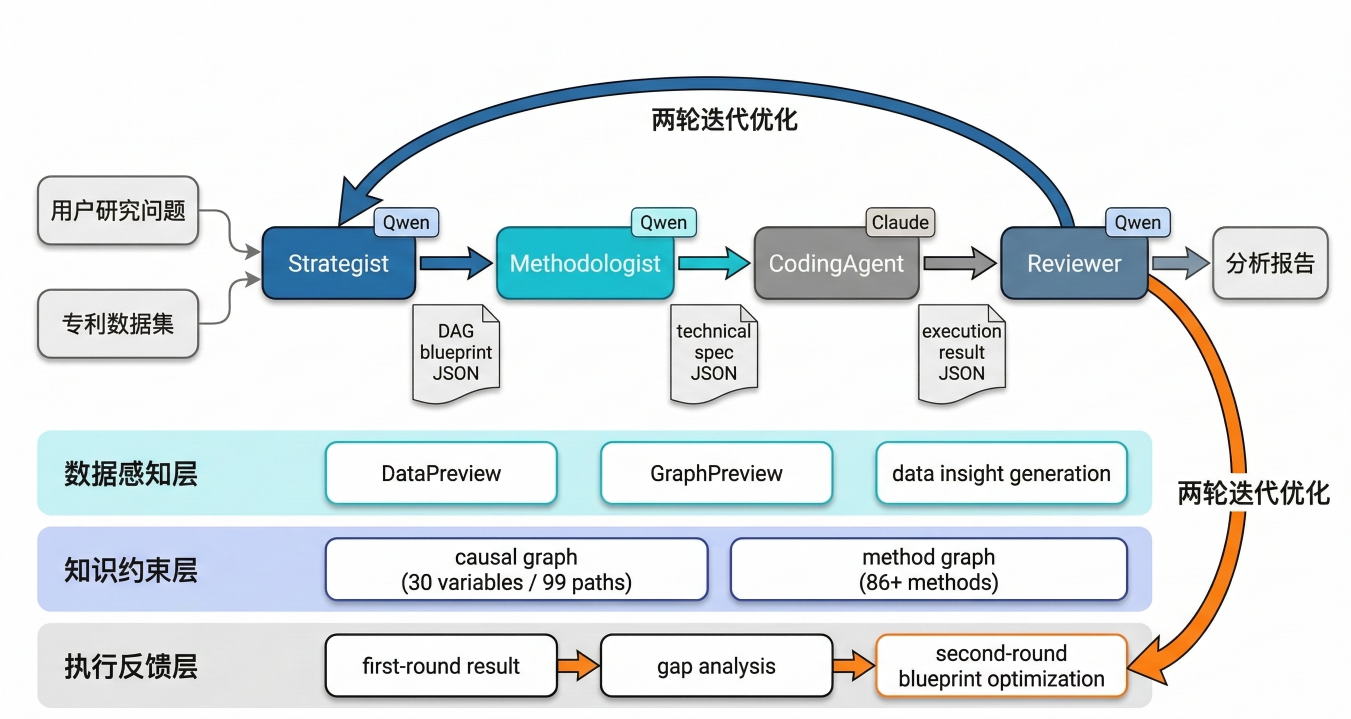
\includegraphics[width=0.95\textwidth]{figures/new_img/图3-1.png}
\caption{系统总体架构图}
\label{fig:3-1}
\end{figure}

各智能体职责与输入输出如下：

\begin{enumerate}[(1)]
\item Strategist（规划智能体）：接收用户研究问题，调用数据感知模块与双图谱模块，输出结构化 DAG 分析蓝图。蓝图节点包括任务目标、输入输出变量、方法建议和参数配置。该智能体是系统的核心决策者，其输出质量直接决定后续分析深度。换言之，Strategist 主要承担“研究设计者”的角色，负责在多种可行路径中选择最值得执行的分析主线。
\item Methodologist（方法规格化智能体）：将蓝图节点进一步规格化，生成可执行技术说明，包括函数签名、输入契约、变量约束、参数要求与预期输出类型。该智能体充当规划层与执行层之间的“翻译器”，将高层研究意图转化为精确的技术合同。其存在的意义在于避免 CodingAgent 直接面对过于抽象的规划描述，从而降低代码生成阶段的歧义与偏差。
\item CodingAgent（执行智能体）：基于规格自动生成 Python 分析代码并在沙箱环境中执行；若执行失败（如列名不存在、类型错误、统计包调用异常），利用错误反馈进行迭代修复，最多重试 15 轮。该智能体承担的是“工程实现者”角色，其核心任务并非仅仅写出代码，而是确保分析任务能够在真实数据环境中被稳定执行并返回结构化结果。
\item Reviewer（评审智能体）：对执行结果进行结构一致性检查与语义有效性评估，生成最终分析报告并返回关键证据链。该智能体相当于系统中的“质量把关者”，负责判断执行结果是否真正回答了原始研究问题，以及当前证据是否足以支撑相应结论。
\end{enumerate}

在智能体选型上，系统采用“双模型分工”策略：通义千问（Qwen）负责文本规划与评审任务（Strategist、Methodologist、Reviewer），Claude 负责代码生成与执行修复任务（CodingAgent）\cite{zhao2024llm,brown2020language}。这一设计并非简单叠加多个模型，而是基于不同模型在长文本理解、结构化规划、代码生成与错误修复等方面的能力差异进行功能匹配。前者更适合处理研究问题理解、方法组织与结果总结等偏语言规划任务，后者更适合处理程序生成、报错修复和执行迭代等偏工程实现任务。该组合将“文本规划稳定性”和“代码生成准确性”分别优化，降低单模型在全流程任务中的能力短板，也使系统在整体上具备更好的鲁棒性与任务适配能力。

\subsubsection{三个基础能力层}

在智能体链路之外，系统包含三个基础能力层。若将四智能体流水线理解为系统的“决策与执行主体”，那么这三个能力层则构成其稳定运行所依赖的底层支撑环境。它们分别从数据事实供给、领域知识约束和执行结果回流三个方面，为智能体链路提供输入依据、边界条件和迭代动力。这样的设计避免了智能体仅凭自然语言上下文完成复杂分析规划，也使系统从“模型驱动”进一步转向“模型 + 数据 + 知识 + 反馈”共同驱动。

\textbf{数据感知层}：DataPreview 与 GraphPreview 分别处理统计关系与图结构关系，输出结构化事实。DataPreview 负责列类型识别、跨列相关系数计算、分组对比和时间趋势检测；GraphPreview 负责自动检测多值字段、构建图结构并运行标准图算法（社区检测、中心性分析等）。两个模块的输出合并后驱动 LLM 生成“数据洞察”，为蓝图规划提供证据基础。该能力层解决的是“系统如何在规划前理解当前数据”的问题，其价值在于将原本隐含在原始表格和网络结构中的信息显式化、结构化，从而使后续智能体能够围绕真实数据特征而不是抽象问题描述开展分析。

\textbf{知识约束层}：因果图谱编码了专利计量领域的核心变量关系（30 个变量、99 条因果路径），提供假设生成的 6 种策略模板；方法图谱包含 86 种以上分析方法，提供变量测量和统计分析的推荐方案。两类图谱均基于 Web of Science 检索获取的 800 余篇专利分析领域文献，经系统性编码提取而成（详见第四章 4.2.6 节）。两类图谱在 Strategist 阶段协同使用：先由因果图谱确定“研究什么”，再由方法图谱确定“怎么做”\cite{pan2024unifying,liu2016knowledge}。该能力层解决的是“系统如何避免规划完全依赖语言模型自由生成”的问题，通过将领域经验、变量关系和方法路径组织为可调用的结构知识，为分析方案提供理论边界与方法指引。

\textbf{执行反馈层}：第一轮执行结果经差距分析后回流 Strategist，用于第二轮蓝图优化。差距分析自动评估第一轮“已回答”和“未充分回答”的问题，并提出深化策略（如增加控制变量、引入非线性模型、补充机制检验等）。该能力层解决的是“系统如何根据实际结果持续修正方案”的问题，使整个工作流不再停留于一次性规划，而具备基于执行证据进行自我修补和逐步深化的能力。

从整体关系看，数据感知层提供“事实输入”，知识约束层提供“结构边界”，执行反馈层提供“修正依据”。三者共同嵌入四智能体流水线之中，使系统在前端具备感知能力，在中端具备约束能力，在后端具备学习式优化能力。这种设计使得系统总体上不只是一个多智能体协作框架，而是一个具备数据支撑、知识支撑与反馈支撑的分析决策系统。

\subsubsection{模块间数据流}

从“用户输入研究问题”到“系统输出分析报告”，整体流程被组织为一条单向流水线，各模块间通过结构化 JSON 传递信息，既保证了链路的清晰可视，又便于在任意阶段插入人工检查或替换实现模块。

\begin{enumerate}[(1)]
\item 用户输入研究问题（字符串）和数据文件路径后，DataPreview 和 GraphPreview 并行处理数据集，分别输出统计摘要文本和图结构特征文本。该步骤完成的是对原始数据的“感知与表征”，将难以直接纳入提示词的大规模表格与网络，压缩为可被 LLM 理解的结构化事实输入。
\item Strategist 接收上述文本、用户目标和双图谱查询结果，输出 DAG 蓝图 JSON。蓝图中每个任务节点的 \texttt{columns\_to\_load} 字段经过列名校验，确保引用的列在数据集中实际存在。此时系统完成了从“研究问题 + 数据事实 + 领域知识”到“可执行任务图”的映射，为后续自动化实现提供清晰的任务分解和依赖关系。
\item Methodologist 逐个接收蓝图节点，输出技术规格 JSON。技术规格包含函数签名、输入验证逻辑和预期输出结构，起到“自然语言规划”和“可执行代码”之间的中间契约作用，使 CodingAgent 可以在不反复理解上游语义的前提下，专注于代码生成与调试。
\item CodingAgent 基于技术规格生成 Python 代码并执行，输出结果 JSON 文件。若执行失败，错误信息反馈给 CodingAgent 触发修复循环。该阶段将抽象分析任务具体化为脚本级操作，并通过自动修复机制提高执行成功率，减少因代码错误导致的整条流水线中断。
\item Reviewer 接收所有任务的执行结果，输出评审报告。在两轮迭代模式下，第一轮的评审结果和原始执行输出反馈给 Strategist，驱动第二轮蓝图生成，使系统具备在“规划—执行—评审”闭环内自我迭代的能力。
\end{enumerate}

该流水线模式的关键优势是\textbf{中间产物完全可追踪}：蓝图 JSON、技术规格、Python 代码和执行结果均有独立文件，便于事后审计和复跑验证\cite{hong2024metagpt}。此外，由于每一阶段均采用明确的数据结构进行输入输出，系统可以在不改动整体架构的前提下替换局部实现（如更换 LLM 或执行环境），增强了工程上的可维护性与可扩展性。

\subsection{数据感知方案生成流程}

本节阐述系统的核心创新——数据感知方案生成的设计思路。

传统 LLM 分析系统的规划过程为"问题$\rightarrow$方案"，即仅根据问题语义生成分析任务，不考虑当前数据集的具体特征。该模式的主要问题是方案容易模板化——对不同数据集生成高度相似的分析路径\cite{guo2024dsagent,hong2025data}。

本文提出的数据感知流程将规划过程改为"问题 + 数据事实$\rightarrow$洞察$\rightarrow$方案"，如图 3-2 所示。

% 图3-2
\begin{figure}[htbp]
\centering
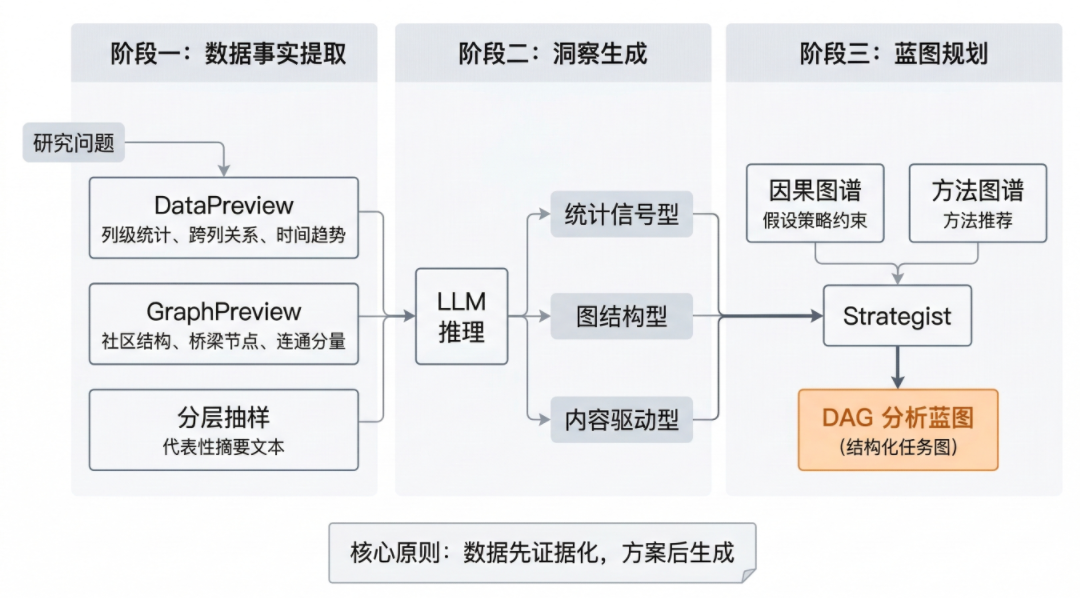
\includegraphics[width=0.95\textwidth]{figures/new_img/图3-2.png}
\caption{数据感知方案生成流程图}
\label{fig:3-2}
\end{figure}

具体分为三个阶段：

\textbf{阶段一：数据事实提取}。DataPreview 提取列级统计和跨列关系（相关系数、分组均值差异、时间趋势），GraphPreview 提取网络结构特征（社区、桥梁节点、连通分量），分层抽样提供代表性摘要文本。该阶段的输出是纯粹的结构化事实，不包含任何语义解读。
  
\textbf{阶段二：洞察生成}。将阶段一的三类输出（统计特征、图结构、摘要样本）合并为 LLM 提示词，驱动 LLM 生成可检验的研究洞察。每条洞察包含具体的数据观察（必须引用数字）、可检验假设、涉及列名和建议方法。洞察分为统计信号型、图结构型和内容驱动型三类。
  
\textbf{阶段三：蓝图规划}。Strategist 以洞察为主驱动、以双知识图谱为辅助约束，生成 DAG 蓝图。该阶段选择 2-3 条核心洞察作为分析起点，结合因果图谱的假设策略和方法图谱的方法推荐，设计具体的分析任务链。

该过程的核心设计原则是\textbf{数据先证据化、方案后生成}：系统先将数据转化为结构化证据，再基于证据设计方案，而非反过来。

\subsection{两轮迭代优化设计}

在前述多智能体架构与基础能力层之上，系统进一步引入两轮迭代优化机制，将整体行为从"一次性生成"改为"反馈驱动生成"，整体流程如图 3-3 所示。该机制的核心思想是把传统实证研究中"探索—验证"的两阶段范式显式编码进自动化流水线，使系统能够围绕首轮结果进行针对性深化，而非简单重复同类分析。

% 图3-3
\begin{figure}[htbp]
\centering
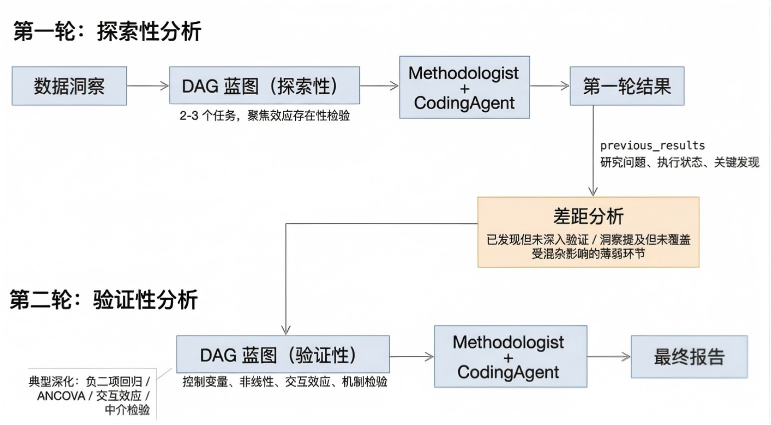
\includegraphics[width=0.95\textwidth]{figures/new_img/图3-3.png}
\caption{两轮迭代优化流程图}
\label{fig:3-3}
\end{figure}

设计思路如下：

\textbf{第一轮（探索性分析）}：基于数据洞察生成初始 DAG 蓝图，通常包含 2-3 个任务，聚焦效应存在性检验（如"X 是否显著影响 Y"）。该轮的目标是快速建立基础变量关系图谱并发现初步信号，为后续集中资源在"最有前景的关系"上提供筛选依据。

\textbf{中间环节（差距分析）}：系统自动评估第一轮结果，识别三类缺口：（1）已发现但未深入验证的信号；（2）洞察中提及但第一轮未覆盖的分析方向；（3）第一轮结论可能受混杂因素影响的薄弱环节。差距分析结果形成第二轮的规划约束，从而避免第二轮重新"从零规划"，而是围绕已发现的问题链路进行有约束的深化。

\textbf{第二轮（验证性分析）}：基于差距分析生成深化 DAG 蓝图，通常引入更多控制变量、非线性模型（如负二项回归替代 OLS）、交互效应检验或机制路径分析（如中介效应检验）。该轮的目标是将分析从"效应是否存在"提升至"效应的机制、路径和边界条件"，使最终结论在因果解释力度和稳健性上更接近实证研究常规标准。

两轮之间的信息传递通过 \texttt{previous\_results} 参数实现，包含第一轮各任务的研究问题、执行状态和关键发现。该方法确保第二轮方案基于第一轮的实际证据而非预设假设。

选择两轮而非单轮或更多轮的设计依据如下。首先，从科学研究方法论角度，"探索—验证"的两阶段范式是实证研究的经典结构：第一阶段建立初步假设并收集证据，第二阶段在控制混杂变量的条件下验证和深化假设\cite{basberg1987patents,trajtenberg1990penny}。该结构既避免了单轮分析因缺乏反馈而产生的浅层化问题，也避免了过多轮次导致的分析主题发散。其次，从边际收益角度，第一轮通常覆盖最显著的变量关系和主效应，第二轮基于差距分析引入控制变量、非线性检验和机制验证，分析层次从"效应发现"提升至"机制解释"。

若引入第三轮，新增信息的边际贡献将显著递减，因为核心假设和主要变量关系已在前两轮中被充分探索。最后，从工程成本角度，每轮涉及 LLM 规划调用、代码生成与执行、结果评审等完整流水线，计算开销随轮次线性增长，两轮在分析深度与资源消耗之间取得了合理平衡。

\subsection{典型应用场景映射}

为验证系统通用性，本文选取三类专利计量场景作为标准应用模板，覆盖“因果效应识别—结构与演化—跨主体比较”三种常见研究取向。每一类场景均通过双图谱检索和数据感知流程自动生成任务图，以检验系统在不同问题结构下的适配能力。

场景一：技术影响力驱动因素分析。目标是识别哪些技术与组织变量显著影响专利影响力，并验证可能机制。系统重点关注因变量定义、控制变量设置、非线性与中介效应识别。该场景对应因果图谱中的"技术影响力"出发点，涉及回归分析与假设检验方法\cite{basberg1987patents,trajtenberg1990penny}，用于检验系统在典型“投入—产出”因果分析任务上的规划与执行能力。

场景二：技术融合趋势识别。目标是识别跨 IPC 部类融合模式与演化趋势。系统重点关注融合度量构建、网络社区结构识别、时间趋势与子群差异检验。该场景充分利用 GraphPreview 的 IPC 共现网络分析能力\cite{daim2006forecasting,zhu2014patent}，用于评估系统在“结构—演化”类网络分析问题上的感知与洞察生成效果。

场景三：国家竞争态势评估。目标是比较不同国家在规模、质量、结构控制力上的差异。系统重点关注指标体系构建、国家分层比较、子技术聚类与竞争格局解释。该场景综合利用分组对比统计和多维度指标计算\cite{narin1997increasing,mejia2024patent}，用于检验系统在“多维指标—多主体比较”类任务中的指标整合和解释能力。

三类场景共享同一架构，但任务图结构不同：场景一偏因果识别，场景二偏结构与趋势，场景三偏比较与聚类。该"共框架、异任务"特征不仅验证了系统设计的可扩展性，也表明方案能够在不同问题类型之间复用同一套数据感知与规划机制。

\subsection{本章小结}

本章从设计目标、总体架构、数据感知流程、两轮迭代设计与应用场景五个方面给出了系统设计方案，系统性地回答了"系统要解决什么问题""整体架构如何支撑该目标"以及"在典型专利计量任务中如何落地"的三个核心问题。

\textbf{设计目标层面}，本章明确了四个核心目标：数据感知、知识增强、迭代优化与端到端闭环。这四个目标并非孤立存在，而是共同构成从问题输入到结论输出的完整设计原则。其中，数据感知目标解决了传统 LLM 分析系统"先规划后看数"的倒置流程问题，确保规划阶段建立在对当前数据事实的显式感知之上；知识增强目标通过因果图谱与方法图谱的协同机制，既避免了完全放任大语言模型自由生成，也避免了将领域经验固化为僵化模板；迭代优化目标将复杂专利问题的渐进式分析特点显式编码进自动化流程，支持基于执行反馈的二次规划与差距修补；端到端闭环目标则确保系统不仅输出规划文本，还能转化为可执行代码和最终报告，实现从用户问题到分析结论的完整自动化链路。

\textbf{总体架构层面}，本章提出了"四智能体流水线 + 三个基础能力层"的混合架构。四智能体（Strategist、Methodologist、CodingAgent、Reviewer）通过 LangGraph 状态机编排，形成具有明确职责边界的闭环流水线，将高层研究意图与底层执行实现解耦，减少单一阶段错误向全流程扩散的风险。三个基础能力层（数据感知层、知识约束层、执行反馈层）分别从数据事实供给、领域知识约束和执行结果回流三个方面，为智能体链路提供输入依据、边界条件和迭代动力。这种设计使得系统从"模型驱动"进一步转向"模型 + 数据 + 知识 + 反馈"共同驱动，避免了智能体仅凭自然语言上下文完成复杂分析规划的问题。

\textbf{核心创新机制层面}，本章提出了两个关键设计：数据感知方案生成流程与两轮迭代优化机制。数据感知流程将传统"问题$\rightarrow$方案"的单向规划改为"问题 + 数据事实$\rightarrow$洞察$\rightarrow$方案"的三阶段流程，核心设计原则是"数据先证据化、方案后生成"，使系统能够围绕真实数据特征而不是抽象问题描述开展分析。两轮迭代优化机制将整体行为从"一次性生成"改为"反馈驱动生成"，第一轮聚焦效应存在性检验，第二轮基于差距分析引入控制变量、非线性检验和机制验证，使分析层次从"效应发现"提升至"机制解释"。

\textbf{与第二章研究不足的对应关系}，本章设计方案直接回应了第二章归纳的三个核心问题：第一，针对"数据感知缺失"问题，通过 DataPreview 与 GraphPreview 模块实现数据事实的前置提取与结构化表征；第二，针对"知识约束不足"问题，通过双知识图谱协同机制（因果图谱约束假设合理性，方法图谱约束方法可执行性）提供结构化知识引导；第三，针对"迭代优化缺失"问题，通过两轮迭代机制与差距分析实现基于执行反馈的渐进式深化。

\textbf{核心结论}，仅有多智能体分工不足以保证高质量分析，必须引入数据感知前置、双图谱协同与迭代反馈机制，才能形成面向专利计量问题的稳定自动化框架。具体而言，数据感知层将"先看数据再规划"制度化，知识约束层将"假设合理性"和"方法可执行性"结构化，迭代反馈层将"一次性方案"升级为"证据驱动的渐进方案"。典型应用场景部分进一步展示了该框架在不同问题结构下的任务图差异与可扩展性，验证了"共框架、异任务"的设计思路。

下一章将从工程视角展开，给出各模块的实现细节与关键算法流程，展示上述设计原则如何转化为可执行的原型系统。


\section{系统原型实现}

\subsection{系统架构与技术选型}

本系统以 Python 为核心实现语言，运行环境为本地单机（Python 3.x + Conda 虚拟环境），整体采用"LLM 代理 + 传统 Python 库"的混合架构。上层通过 LangGraph\cite{langgraph2024} 组织多智能体状态机流程，下层则由 pandas、NetworkX 等库完成具体的数据处理与图计算。LangGraph 提供显式的节点—边定义和有向图执行模型，便于将第三章提出的 DAG 蓝图和多智能体分工直接映射为可执行的工程状态机。

在模型选型上，系统采用"双模型分工"策略：通义千问（Qwen）负责规划和评审，Claude 负责代码生成和执行修复。该组合的工程出发点是将"文本规划稳定性"和"代码生成能力"分开优化，降低单模型在全流程任务中的能力短板\cite{zhao2024llm,brown2020language}。具体做法上，Strategist、Methodologist 与 Reviewer 的提示词均针对 Qwen 调优，强调长文本理解、结构化输出和批判性评估；CodingAgent 的提示词则针对 Claude 调优，强调类型约束、异常处理和最小可复现单元。通过在架构层明确职责边界，可以在不改动代码框架的前提下替换底层大模型，实现平滑升级。

系统主模块代码路径如下。工作流编排在 \texttt{src/core/\allowbreak workflow.py}，规划模块在 \texttt{src/agents/\allowbreak strategist.py}（约 1520 行），方法规格化模块在 \texttt{src/agents/\allowbreak methodologist.py}，执行模块在 \texttt{src/agents/\allowbreak coding\_agent\_v4\_2.py}，评审模块在 \texttt{src/agents/\allowbreak reviewer.py}。数据感知由 \texttt{src/utils/\allowbreak data\_preview.py}（602 行）与 \texttt{src/utils/\allowbreak graph\_preview.py}（451 行）提供，知识约束由 \texttt{src/graphs/\allowbreak causal\_graph\_query.py} 与 \texttt{src/graphs/\allowbreak method\_graph\_query.py} 提供。各模块之间通过 JSON 或 Python 字典进行解耦传递，使得任何一个模块都可以在保持接口不变的前提下独立重构。

从工程职责角度，系统采用"规划—规格—执行—评审"四段式流水线，每段均有结构化 JSON 输入输出（整体架构参见图 \ref{fig:3-1}）。该方法使系统不仅能产出结果，也能产出中间证据链，便于复核与追踪\cite{hong2024metagpt,langgraph2024}。同时，结合前一章提出的三层基础能力结构，系统在流水线两端分别插入 DataPreview/GraphPreview 的数据感知模块与差距分析模块，将"数据事实—规划蓝图—执行结果"连接为闭环，有利于后续在日志与监控层面实现细粒度的错误诊断与性能分析。

\subsection{系统核心模块实现}

DataPreview 的目标是将"数据事实"前置到方案规划阶段。模块输入为 pandas DataFrame，输出为结构化预览对象，包含列类型画像、基础统计、跨列统计和抽样摘要四部分。

\subsubsection{列语义识别与类型画像}

列语义识别与类型画像是数据感知模块的入口环节，其目标是将原始数据表中“面向存储的列名”转化为“面向分析的语义标签”。系统首先识别数值列、分类列、日期列和文本列，并为每列生成质量摘要（缺失率、唯一值数、分布形态），为后续跨列统计和图构建提供必要前提。

在专利数据场景下，列名往往为中文短语且包含括号、下划线等符号，直接输入给 LLM 易产生歧义。为此，模块内置了一套列语义映射表，覆盖 30 余个常见专利字段，将列名映射为分析语义描述。例如：

\begin{table}[htbp]
\centering
\caption{列语义映射示例}
\label{tab:column-mapping}
\begin{tabular}{@{}ll@{}}
\toprule
原始列名 & 语义描述 \\ \midrule
被引用专利数量 & 被引用次数（数值维度，反映专利影响力） \\
IPC分类号 & 技术领域分类（多值分隔符列，可构建共现网络） \\
申请日 & 申请时间（日期维度，用于时间趋势分析） \\
发明人 & 发明人姓名（多值列，可构建合作网络） \\ \bottomrule
\end{tabular}
\end{table}

该映射表在实现上采用"规则模板 + 自适应匹配"的方式：一方面通过精确匹配和正则表达式覆盖常见字段（如"被引用专利数量（次）"与"被引用次数"归为同一语义），另一方面在找不到精确规则时回退到基于关键词的模糊匹配，并将低置信度映射显式标注在预览结果中。这样设计使得后续 LLM 在生成分析方案时能够直接理解每列的分析用途，避免因列名歧义导致的错误，同时保留人工复核和扩展映射表的空间。

\subsubsection{跨列统计关系抽取}

跨列统计是 DataPreview 的核心功能，用于自动发现数据中的变量关系线索，相当于在"列语义已对齐"的基础上，对潜在的变量间关系进行一次自动勘探。模块实现三类跨列统计：

\begin{enumerate}[(1)]
\item \textbf{数值列 Pearson 相关系数}。对所有数值列两两计算相关系数，过滤 $|r| > 0.1$ 的显著关联，按绝对值降序保留前 20 对。该步骤的作用是为后续假设生成提供"哪些变量之间存在线性关联"的定量线索，并避免把注意力浪费在相关性极弱的变量对上。
\item \textbf{分类列分组对比}。对低基数分类列（唯一值 $\leq$ 50），按 Top 5 类别分组计算核心数值列均值差异。例如，按"法律状态"分组计算"被引用专利数量"的均值差异，可以发现"授权|权利转移"状态的专利平均被引量是否高于普通授权专利。通过限制类别数和核心数值列数量，模块在保持信号代表性的同时控制输出长度，便于 LLM 在有限上下文中理解。
\item \textbf{时间趋势检测}。自动检测日期列，按年聚合计算核心数值列的年度均值趋势。该信号可用于发现被引量的时间衰减效应等，也为后续构造时间虚拟变量或分段回归提供依据。
\end{enumerate}
跨列统计的处理流程如算法 4-1 所示，整体数据流见图 4-1：

\begin{algorithm}[H]
\caption{跨列统计计算}
\KwIn{DataFrame df, 列类型画像 profile}
\KwOut{跨列统计结果 result}

numeric\_cols $\leftarrow$ 从 profile 中提取所有数值列\;
\tcp{相关系数计算}
corr\_matrix $\leftarrow$ df[numeric\_cols].corr(method='pearson')\;
pairs $\leftarrow$ 提取 $|r| > 0.1$ 的列对，按 $|r|$ 降序排列，取前 20 对\;
result.correlation\_pairs $\leftarrow$ pairs\;
\tcp{分组对比}
cat\_cols $\leftarrow$ 从 profile 中提取唯一值 $\leq$ 50 的分类列（取前 5 个）\;
core\_numeric $\leftarrow$ 排除 ID 类列的数值列（取前 3 个）\;
\ForEach{cat\_col in cat\_cols}{
    top\_cats $\leftarrow$ cat\_col 出现频率最高的 5 个类别\;
    \ForEach{num\_col in core\_numeric}{
        grouped\_means $\leftarrow$ df[cat\_col $\in$ top\_cats].groupby(cat\_col)[num\_col].mean()\;
        result.group\_comparisons.append(\{group\_by, metric, values\})\;
    }
}
\tcp{时间趋势}
date\_col $\leftarrow$ 检测含日期关键词的列\;
years $\leftarrow$ pd.to\_datetime(date\_col).dt.year\;
\ForEach{num\_col in core\_numeric}{
    yearly\_means $\leftarrow$ df.groupby(years)[num\_col].mean()\;
    result.time\_trends.append(\{metric, by\_year\})\;
}
\Return{result}\;
\end{algorithm}
% 图4-1
\begin{figure}[H]
\centering
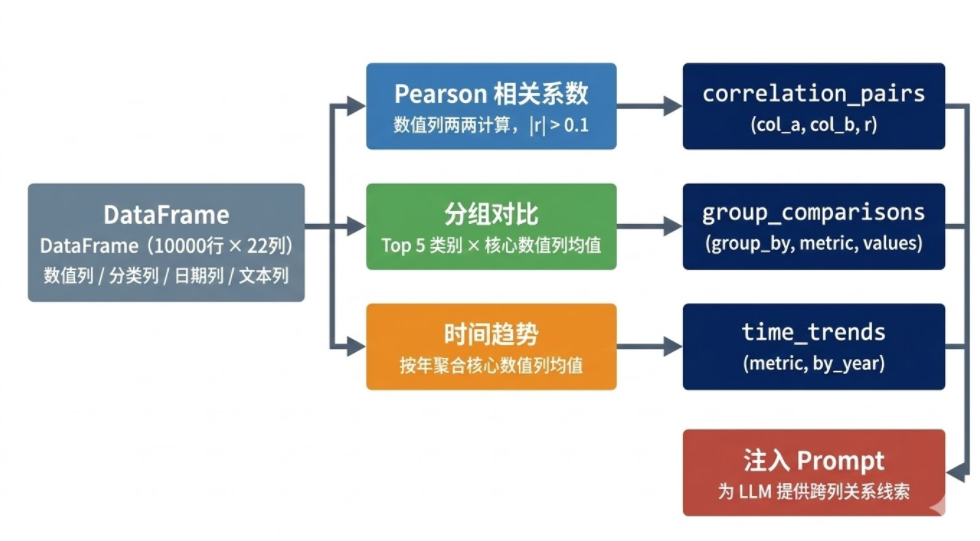
\includegraphics[width=0.95\textwidth]{figures/new_img/图4-1.png}
\caption{跨列统计数据流图}
\label{fig:4-1}
\end{figure}

\subsubsection{内容样本的分层抽样}

为让 LLM 了解专利的技术内容分布，仅依赖数值特征和 IPC 结构仍然不够，需要提供少量有代表性的摘要原文。模块按 IPC 分部（首字符 A-H）对摘要进行分层抽样，每部最多采 5 条、总计不超过 30 条，每条截断至 300 字符，使提示词在长度可控的前提下覆盖主要技术领域。

具体实现中，系统首先基于 IPC 首字符将专利划分为最多 8 个技术分部，对每个分部分别随机抽取不超过 5 条摘要；若某一分部专利数量不足 5 条，则全部纳入样本。为避免极端长摘要挤占上下文窗口，所有摘要在句子边界附近截断至约 300 字符，并保留 IPC 及基础元数据标签，便于 LLM 理解样本所属领域。

使用固定随机种子（random\_state=42）保证可复现。相比简单的全局随机抽样，分层抽样确保各技术领域均有代表性样本，降低了主题偏置，也降低了 LLM 将少数高频领域误判为总体分布的风险。

\subsubsection{图结构预览模块（GraphPreview）}

GraphPreview 用于捕捉 DataPreview 难以表达的网络结构信息，是数据感知模块中面向"关系结构"的补充维度。专利数据中存在大量多值关系字段（如 IPC 分类号、发明人、引用专利），这些字段天然可以构建为图，揭示共现关系和协作模式，从而为后续的社区发现、结构洞察和局部子网络分析提供基础。

\noindent\textbf{1.自动图构建策略}

模块首先扫描 DataFrame 中所有含分隔符的列，将其识别为"可构图候选列"。随后通过元素类型分类器判断列内元素的类型，决定构建何种图，自动构图逻辑如图 4-2 所示。

% 图4-2
\begin{figure}[H]
\centering
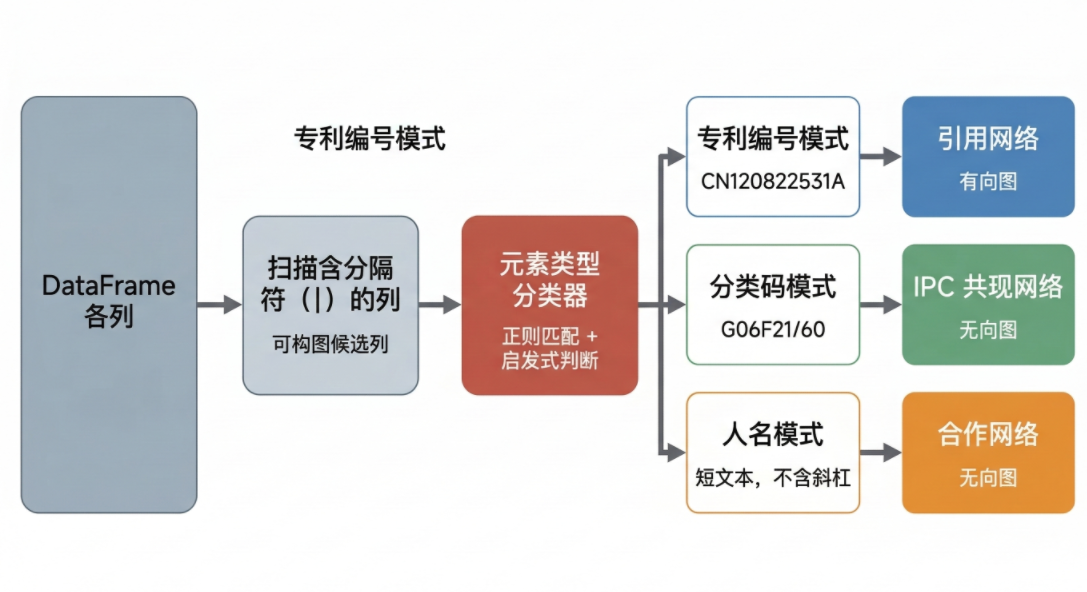
\includegraphics[width=0.95\textwidth]{figures/new_img/图4-2.png}
\caption{自动构图逻辑图}
\label{fig:4-2}
\end{figure}

分类器对采样元素进行正则匹配和启发式判断：

\begin{enumerate}[(1)]
\item 若元素匹配专利编号模式（如 CN120822531A），构建\textbf{引用网络}
\item 若元素匹配分类码模式（如 G06F21/60），构建\textbf{共现网络}
\item 若元素为短文本且不含斜杠，判定为人名，构建\textbf{合作网络}
\end{enumerate}

在实测中，系统从数据集自动构建了 6 个图：发明人合作网络、IPC 共现网络、引用网络等，无需用户显式指定"要看哪张图"。这一策略减少了使用门槛，同时保证了不同数据集在图结构分析阶段的处理流程具有可比性。

\noindent\textbf{2.分层图算法策略}

为兼顾信息密度与计算性能，模块采用分层计算策略。当图规模较小时（节点数 $\leq$ 10,000），完整计算以下指标：Louvain 社区检测（使用 python-louvain 库，固定 random\_state=42，输出社区数量、各社区规模和每社区 Top 3 代表节点）、介数中心性（对大图使用 k=500 近似采样降低复杂度，输出 Top 10 桥梁节点）、连通分量统计（输出最大连通分量占比和孤立节点数）、度分布统计（输出平均度、最大度和度分布分位数）。

当图规模超过阈值（LARGE\_GRAPH\_\allowbreak THRESHOLD = 10,000）时，跳过社区检测和介数中心性计算，仅保留度分布统计，避免 O($n^2$) 级操作导致规划阶段阻塞。这样可以在保证"大致结构特征可见"的前提下，将最耗时的运算限制在中小规模图上，对大规模数据集保持可接受的响应时间。

\begin{algorithm}[H]
\caption{图结构预览生成}
\KwIn{DataFrame df}
\KwOut{图结构指标集合 metrics}

candidate\_cols $\leftarrow$ 检测含分隔符(|)的列\;
\ForEach{col in candidate\_cols}{
    elem\_type $\leftarrow$ ClassifyElements(col) \tcp{patent\_id | classification | name}
    G $\leftarrow$ BuildGraph(col, elem\_type) \tcp{构建对应类型的图}
    \eIf{$|V(G)| > 10000$}{
        metrics[G] $\leftarrow$ \{degree\_distribution\} \tcp{仅度分布}
    }{
        communities $\leftarrow$ Louvain(G, random\_state=42)\;
        centrality $\leftarrow$ BetweennessCentrality(G, k=500)\;
        components $\leftarrow$ ConnectedComponents(G)\;
        metrics[G] $\leftarrow$ \{communities, centrality, components, degree\_distribution\}\;
    }
}
\Return{metrics}\;
\end{algorithm}

模块的关键设计原则是\textbf{只输出结构化事实，不做语义解读}。例如，输出"节点 H04L9/40 的介数中心性为 0.31"，而不输出"H04L9/40 是技术桥梁"——后者的判断由 LLM 在洞察生成阶段完成。

\subsubsection{数据洞察生成机制}

数据洞察生成是数据感知方案的核心环节，位于"数据预览"和"蓝图规划"之间，负责把前者输出的数值特征、图结构特征和摘要样本综合成面向分析的高层信号。该过程由 Strategist 中的 \path{_generate_data_insights()} 方法实现，将 DataPreview 与 GraphPreview 的输出合并为 LLM 提示词，驱动 LLM 生成结构化的可检验洞察。

\paragraph{洞察生成的 Prompt 设计}

Prompt 设计遵循"输入尽量完备、输出尽量克制"的原则，包含三层输入和严格的输出约束：

\textbf{输入层}：

\begin{enumerate}
\item 数据统计特征（来自 DataPreview 的相关系数、分组对比、时间趋势）
\item 图结构分析（来自 GraphPreview 的社区、中心性、连通分量）
\item 领域摘要样本（来自分层抽样的 20-30 条专利摘要）
\end{enumerate}

\noindent\textbf{约束层}：每条洞察必须引用输入中的具体数字，必须指定可验证的数据列和分析方法，必须归属于三类之一（统计信号型 statistical、图结构型 graph\_structural、内容驱动型 content\_driven），且禁止常识性结论。通过这种硬约束，系统将 LLM 的输出限制在"可检验、可追踪"的范围内，减少空泛描述和模板化结论。

\noindent\textbf{输出格式}：每条洞察包含 7 个字段：

\begin{table}[htbp]
\centering
\caption{数据洞察输出字段说明}
\label{tab:insight-fields}
\begin{tabular}{@{}lp{10cm}@{}} % 使用 lp 格式，l 为左对齐，p 为固定宽度换行
\toprule
字段 & 含义 \\ \midrule
\texttt{id} & 洞察编号（如 I1, I2） \\
\texttt{type} & 洞察类型（statistical / graph\_structural / content\_driven） \\
\texttt{title} & 洞察标题 \\
\texttt{observation} & 具体数据观察（必须引用数字） \\
\texttt{hypothesis} & 可检验假设 \\
\texttt{data\_columns} & 涉及的数据列名 \\
\texttt{analysis\_method} & 建议的分析方法 \\ \bottomrule
\end{tabular}
\end{table}

\paragraph{洞察示例}

在 Q1（技术影响力驱动因素分析）实验中，系统生成的洞察包括（洞察编号由系统按生成顺序自动分配，不同运行间可能不同）：

\begin{quote}
\textbf{I1}（statistical）：近年授权专利被引量骤降——反映技术迭代加速，需在分析中控制专利年龄，否则会混淆真实影响力。
\end{quote}

\begin{quote}
\textbf{I2}（graph\_structural）：H04L9/40 为核心枢纽——可限定分析范围至该 IPC 主导的子网络，提升假设检验的针对性。
\end{quote}

这些洞察将作为 Strategist 生成 DAG 蓝图的关键输入：一方面提供"从数据中看见了什么"的具体线索，另一方面在后续假设生成与方案评审阶段，被用于识别常识性结论和缺乏证据支撑的分析路径，从而把第三章提出的创新性约束具体落实到工程实现中。

\subsubsection{双知识图谱实现}

系统使用两类图谱协同约束分析方案的"假设空间"和"方法空间"\cite{pan2024unifying,liu2016knowledge}。与完全依赖 LLM 自由生成相比，图谱的引入将"领域共识"显式化为可查询的结构资源，一方面提高方案的理论合理性，另一方面也便于在不同任务与数据集之间保持方法选择的一致性。

\paragraph{图谱知识来源}

双知识图谱的构建基础来源于专利计量分析领域的学术文献，目标是在"覆盖主流研究范式"与"保持编码成本可控"之间取得平衡。本文以 Web of Science 核心合集数据库为检索平台，使用以下检索策略：

\begin{lstlisting}[basicstyle=\ttfamily\small,frame=single,breaklines=true]
TS=("Patent analysis" OR "Patent mining" OR "Tech mining"
    OR "Patent landscape" OR
    (("Bibliometric*" OR "Scientometric*") AND "Patent"))
\end{lstlisting}

筛选条件限定文献类型为研究论文（Article）和综述（Review Article），学科类别覆盖管理学、信息科学、计算机科学和经济学等相关领域。初步检索获得 1,400 余篇相关文献，经去重和全文可获取性筛选后，成功下载 800 余篇专利分析领域的学术论文，形成图谱构建的文献语料库。

在此基础上，本文通过系统性文献编码提取两类知识：一是专利计量研究中反复出现的变量关系与因果假设（如"技术多样性$\rightarrow$技术影响力"、"企业规模$\rightarrow$专利质量"等），据此构建因果图谱；二是文献中使用的统计分析方法与变量测量方案（如引用网络分析、IPC 共现分析、负二项回归等），据此构建方法图谱\cite{basberg1987patents,trajtenberg1990penny,griliches1990patent,zhu2014patent}。该构建过程确保图谱内容基于领域内广泛认可的研究范式，而非个别研究的偶然选择，也为后续评价系统输出的"理论对齐程度"提供了可追溯的参照系。

因果图谱编码了专利计量领域的核心变量关系，包含 30 个变量和 99 条因果路径，局部示例如图 4-3 所示。图中的有向边表示"在文献中被反复假定或验证的因果方向"，节点属性记录变量类型（如技术属性、组织属性、绩效结果等），便于在规划阶段快速过滤出与当前研究目标相关的子图。

% 图4-3
\begin{figure}[H]
\centering
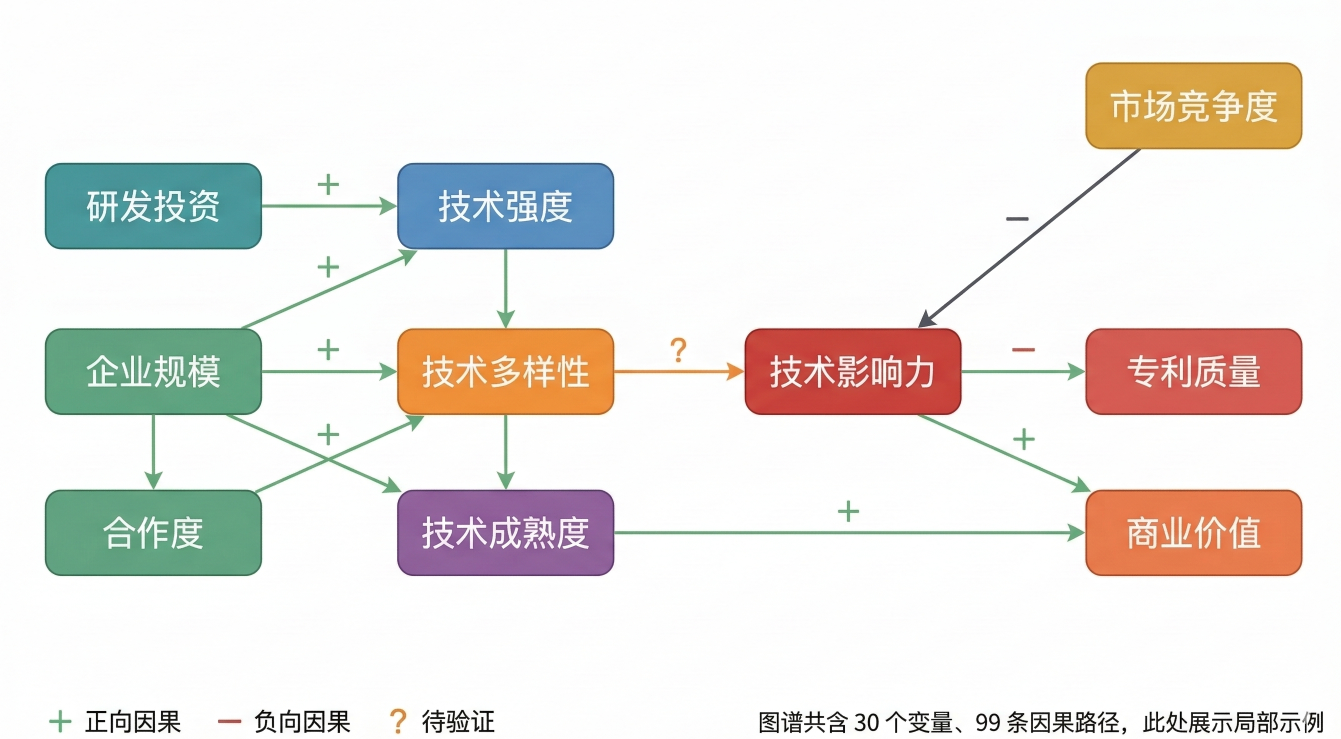
\includegraphics[width=0.95\textwidth]{figures/new_img/图4-3.png}
\caption{因果图谱局部示例}
\label{fig:4-3}
\end{figure}

变量涵盖技术强度、企业规模、研发投资、技术多样性、技术影响力、商业价值等维度。系统在运行时会根据用户研究目标在因果图中检索以目标变量为终点或起点的局部结构，并结合第三章提出的 6 种假设生成策略，对这些结构进行系统性枚举。

图谱提供 6 种假设生成策略模板：

\begin{table}[htbp]
\centering
\caption{因果图谱假设生成策略}
\label{tab:causal-strategies}
\renewcommand{\arraystretch}{1.3} % 适当增加行间距，提升长文本可读性
\begin{tabular}{@{}llp{6cm}@{}} % 根据内容长度调整列宽比例
\toprule
策略 & 核心思路 & 示例 \\ \midrule
理论迁移 & 将已验证理论应用到新场景 & 将“研发投资 $\rightarrow$ 技术产出”路径迁移至专利数据 \\
路径探索 & 发现文献中未充分研究的因果路径 & 探索“技术多样性 $\rightarrow$ 商业价值”的间接路径 \\
边界条件 & 为已知关系寻找调节变量 & 企业规模是否调节“技术多样性”与“影响力”的关系 \\
中介机制 & 揭示 $X \rightarrow M \rightarrow Y$ 的中介效应 & 技术多样性是否通过“技术成熟度”中介影响商业价值 \\
反事实推理 & 生成反直觉假设 & 技术多样性高的专利影响力反而更低？ \\
交互效应 & 探索多变量联合作用 & 研发投资与技术多样性的交互项是否显著 \\ \bottomrule
\end{tabular}
\end{table}

方法图谱包含 86 种以上的分析方法，按两个维度组织：一是变量测量方法（variable\_measurement\_methods），为每个变量 ID 提供推荐的量化方式；二是统计分析方法（statistical\_analysis\_methods），按类型分为回归分析（regression）、中介分析（mediation）、调节分析（moderation）。在工程实现上，两类知识均以可查询的 JSON 结构存储，Strategist 与 Methodologist 可通过变量 ID 和假设类型进行检索与匹配。

方法匹配逻辑：根据假设类型自动推荐适配的分析方法。例如，中介效应假设自动匹配 Bootstrap 中介检验方法；调节效应假设自动匹配层次回归方法。方法匹配示例如图 4-4 所示。通过这种显式映射，系统可以避免出现"用不恰当方法检验特定假设类型"的情况，并在不同运行之间保持方法选择的一致性。

% 图4-4
\begin{figure}[H]
\centering
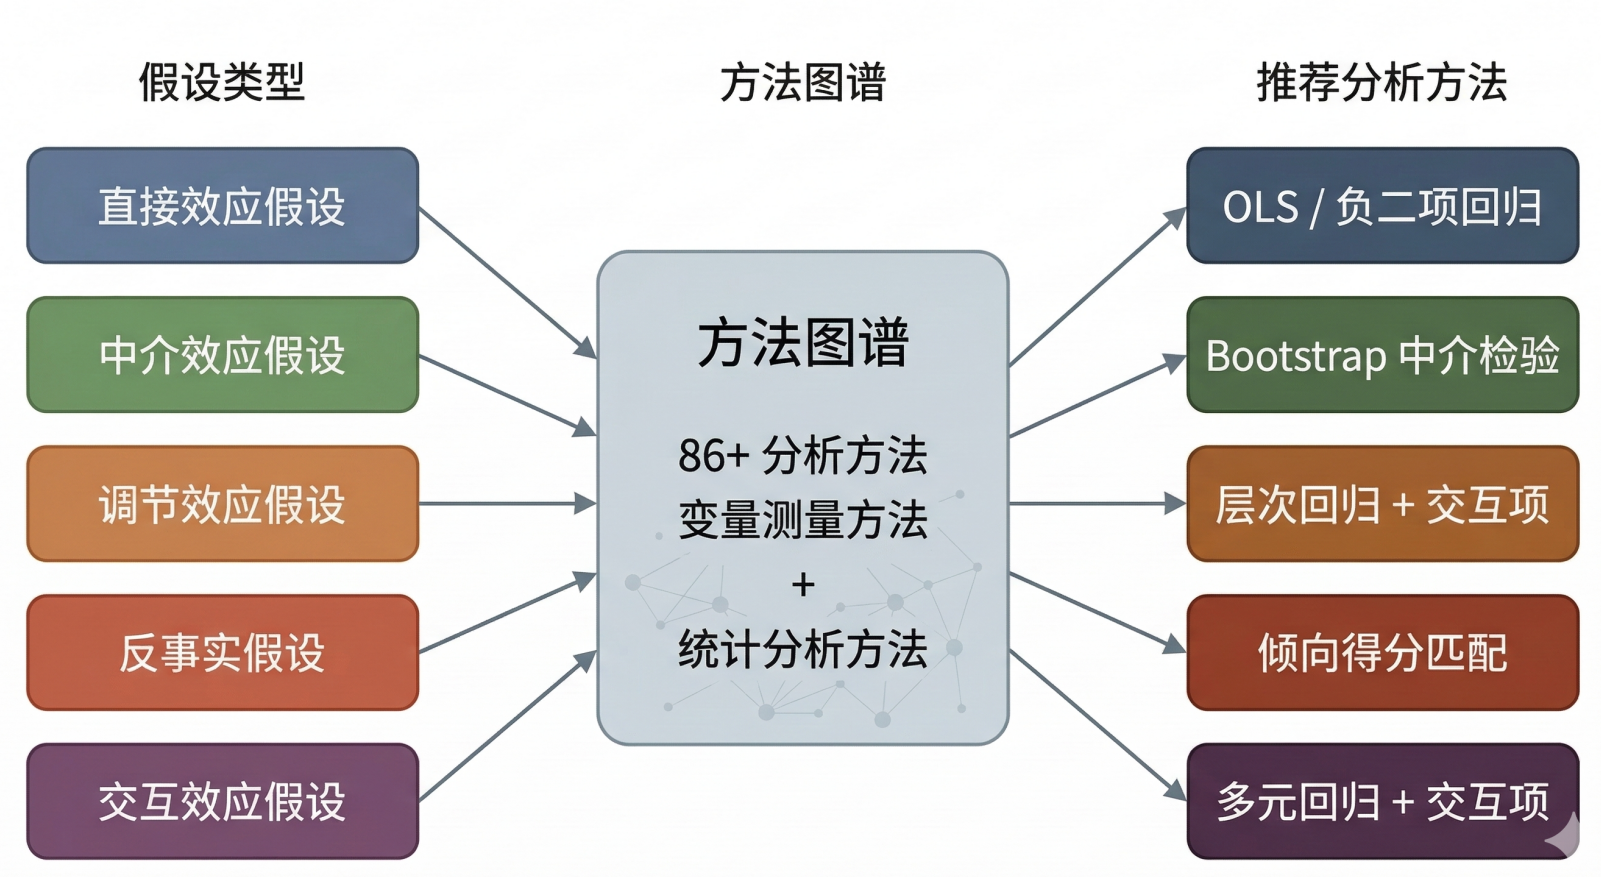
\includegraphics[width=0.95\textwidth]{figures/new_img/图4-4.png}
\caption{方法匹配示例图}
\label{fig:4-4}
\end{figure}

在 Strategist 中，双图谱的使用顺序为：先由因果图谱生成候选假设（确定"研究什么"），再由方法图谱匹配执行方法（确定"怎么做"）。该顺序保证先确定理论合理的研究方向，再确定技术可执行的实现路径，避免出现"先选方法再寻找问题"或"理论合理但工程上难以实现"的方案。此外，双图谱的查询结果会被写入蓝图节点的元数据中，便于 Reviewer 在事后审查某一任务是否真正对应了既有研究范式。

\subsubsection{分析蓝图生成与执行闭环}

\paragraph{DAG 蓝图结构}

Strategist 输出的蓝图为有向无环图（DAG），每个节点代表一个分析任务，是连接"高层研究目标"与"底层可执行代码"之间的核心中间表示。任务节点包含以下字段：

\begin{lstlisting}[basicstyle=\ttfamily\small,frame=single,breaklines=true]
{
"task_id": "task_1",
"task_type": "hypothesis_test",
"question": "技术跨界度对技术影响力是否有负向影响？",
"description": "在H04L9/40子群中进行多元回归...",
"input_variables": [],
"output_variables": ["result_1"],
"dependencies": [],
"implementation_config": {
"data_source": "data/new_data.XLSX",
"sheet_name": "sheet1",
"columns_to_load": ["IPC分类号", "被引用专利数量", "授权日"],
"parameters": {
"core_ipc": "H04L9/40",
"control_vars": ["patent_age", "legal_status_dummies"]
},
"output_format": "json",
"output_file": "outputs/task_1_result.json"
}
}
\end{lstlisting}

节点间通过 \texttt{dependencies} 字段和 \texttt{input\_variables}/\texttt{output\_variables} 字段建立依赖关系，确保任务按正确顺序执行。DAG 结构还支持在出现执行失败时，仅重跑受影响的子图，而无需重复整个流程。

Methodologist 将蓝图节点进一步转化为技术规格，包括函数签名、输入契约、变量约束、参数说明与预期输出类型。该步骤的作用是在 Strategist 的高层规划和 CodingAgent 的底层执行之间建立精确的"合同"。在实现上，Methodologist 会对蓝图中常见的不确定项（如列名模糊、参数范围不清晰）进行补全或显式标注，避免这些模糊性直接传递到代码生成阶段。

CodingAgent 基于技术规格自动生成并执行 Python 代码，执行与纠错流程如图 4-5 所示。系统为每个任务维护独立的日志与输出文件夹，记录原始代码、标准输出、错误栈信息和修复历史，便于后续复盘与人工审查。

% 图4-5
\begin{figure}[H]
\centering
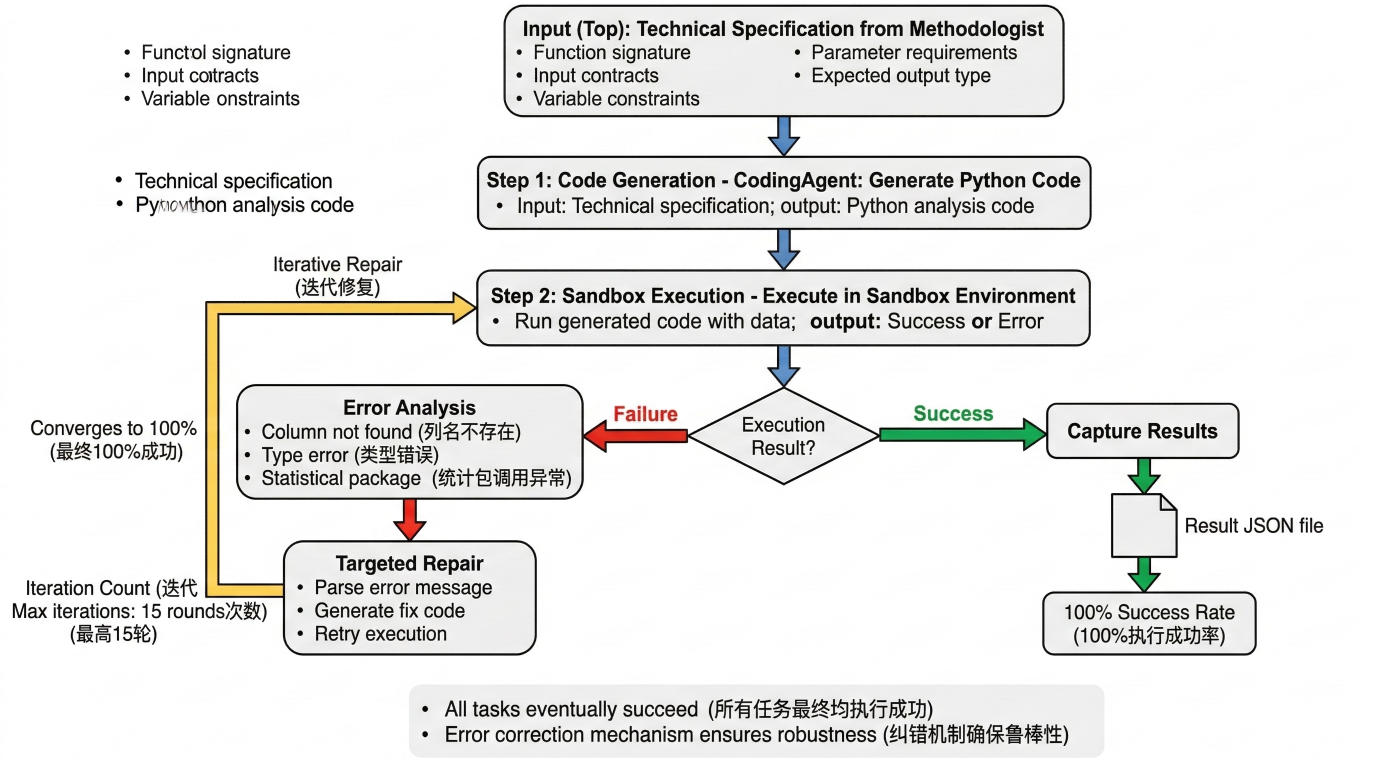
\includegraphics[width=0.95\textwidth]{figures/new_img/图4-5.png}
\caption{执行与纠错流程图}
\label{fig:4-5}
\end{figure}

若执行失败（如缺列、类型错误、统计包调用异常），系统根据错误信息触发定向修复，最多迭代 15 轮。在实验中，所有任务最终均执行成功（成功率 100\%），说明该纠错机制具有足够的容错能力。

Reviewer 对执行结果进行两个维度的评审：结构完整性检查（输出是否包含预期字段）和语义有效性评估（结论是否回答了研究问题）。评审结果用于最终报告生成，并为差距分析和第二轮规划提供输入，相当于在流水线末端增加一道"LLM-as-judge"式的质量闸门。

\subsubsection{两轮迭代机制}

两轮机制通过 \texttt{round} 与 \texttt{previous\_results} 传递上下文，第二轮蓝图由 \texttt{\_generate\_refined\_blueprint()} 方法生成。与第三章的方法论设计相呼应，这里给出了在工程实现层面如何编码"探索—验证"闭环的具体做法。

\paragraph{第二轮蓝图生成流程}

第二轮 Prompt 包含三个额外输入：

\begin{enumerate}
\item 第一轮各任务的执行结果摘要（关键发现、统计量、结论）
\item 差距分析：评估第一轮"已回答"和"未充分回答"的问题边界
\item 深化策略：补充控制变量、增加交互项检验、引入非线性模型
\end{enumerate}

\begin{algorithm}[H]
\caption{两轮规划流程}
\KwIn{用户研究目标 goal, 数据集 data}
\KwOut{两轮分析结果 final\_results}

\tcp{第一轮：探索性分析}
insights $\leftarrow$ GenerateDataInsights(data, goal)\;
blueprint\_1 $\leftarrow$ Strategist(goal, data, insights, round=1)\;
results\_1 $\leftarrow$ Execute(blueprint\_1) \tcp{Methodologist $\rightarrow$ CodingAgent $\rightarrow$ Reviewer}
\tcp{第二轮：验证性分析}
gap $\leftarrow$ AnalyzeGap(results\_1, goal, insights)\;
blueprint\_2 $\leftarrow$ Strategist(goal, data, insights, round=2, previous\_results=results\_1, gap=gap)\;
results\_2 $\leftarrow$ Execute(blueprint\_2)\;
final\_results $\leftarrow$ Merge(results\_1, results\_2)\;
\Return{final\_results}\;
\end{algorithm}

迭代效果与单轮流程相比，两轮机制将系统行为从"一次性生成"改为"反馈驱动生成"。实验中，第二轮常见的新增操作包括：负二项回归替代 OLS（非线性建模）、BERT 主题建模（文本挖掘）、IPC 共现网络特征工程（图结构利用）、交互项检验（机制验证）。这些操作将分析从效应发现提升至机制解释层次，也为系统在报告中给出"第一轮结论在何种条件下仍然成立"提供了证据基础。

\subsection{本章小结}

本章围绕“把第三章的系统设计落到可运行原型”这一目标，给出了系统核心模块的实现细节与关键工程策略，形成了一套从数据预览到方案生成、从自动执行到结果复核的闭环实现路径。

在数据感知层，DataPreview 通过列语义识别、类型画像与跨列统计（相关、分组对比、时间趋势）将“表格事实”压缩为结构化证据；同时结合分层抽样补充专利摘要样本，使规划阶段能够在有限上下文内把握技术内容分布。GraphPreview 作为补充维度，通过自动构图与分层图算法策略提取“关系结构事实”，在中小规模图上输出社区、中心性与连通性等指标，在大规模图上自动降级以控制复杂度，从工程上兼顾了信息密度与响应时间。

在洞察到蓝图的转换层，实现了数据洞察生成机制：通过约束性 Prompt 将统计信号、图结构特征与内容样本综合为可检验洞察，并要求洞察显式引用输入中的具体数字、指明数据列与分析方法，从而抑制空泛表述和常识性结论。该机制使系统的规划不再是“问题语义驱动”，而是以“证据驱动”为主线，为后续 DAG 蓝图生成提供了稳定的起点与边界。

在知识约束层，双知识图谱在工程上被实现为可查询的结构资源：因果图谱用于收缩与组织假设空间，方法图谱用于约束方法选择与变量测量路径。通过“先假设后方法”的协同调用方式，系统能够在保持可执行性的前提下，将领域共识嵌入到蓝图元数据中，并支持在不同任务之间复用一致的约束逻辑，提升方案的可比性与可复核性。

在执行与迭代层，本章实现了“规划—规格—执行—评审”的闭环流水线，并在其上叠加两轮迭代机制。第一轮用于快速建立主效应与关键结构信号，差距分析对未覆盖方向与薄弱证据进行诊断，第二轮则围绕证据缺口引入控制变量、非线性建模、交互效应或机制检验，推动分析从“效应发现”提升到“机制解释与边界条件”的层次。由于蓝图、技术规格、代码与结果均以结构化文件持久化保存，系统具备较好的追踪性与可复现性，也为后续开展对比实验与消融评估提供了可靠的工程基座。

本章所实现的 DataPreview/GraphPreview、数据洞察生成、双知识图谱与两轮迭代机制共同构成可复核、可迭代的自动分析原型，为第五章的实验与评估提供了可操作的技术基础与过程证据链。

\section{实验与评估}

\subsection{实验设计}

本章主要回答三个问题：其一，数据感知模块是否能够稳定提升方案针对性与证据耦合程度；其二，双知识图谱在完整系统中是否提供可观察的正向贡献；其三，两轮迭代是否能够在保持可执行性的同时进一步提升分析深度与结论质量。为保证结论可归因，本文采用“渐进叠加主线 + 组件消融补强 + 重复实验验证”的实验组织方式：主实验负责解释系统为何逐步变好，消融实验负责解释完整系统中各关键组件的独立作用，重复实验则用于检验这些结论在多次独立运行下是否仍然成立。

\subsubsection{数据集说明}

本研究以智慧芽（PatSnap）全球专利数据库作为核心数据来源。该数据库覆盖全球 170 余个国家和地区的专利信息，为刻画全球数据流通安全技术博弈格局提供了广阔且权威的时空视角。数据采集的时间跨度设定为 1972 年至 2026 年初（检索截止日期为 2026 年 1 月），旨在从技术演进的长周期出发，捕捉数据流通安全相关技术范式的关键跃迁。之所以选取专利作为观测载体，一方面在于其作为法律保护客体具有较高权威性，另一方面专利文献中结构化的权利要求书和技术说明书，为后续基于大模型的深度语义挖掘提供了高质量、标准化的语料基础。

在检索策略上，本研究针对数据流通安全的多学科交叉特性，构建了“关键词 + 国际专利分类号（IPC）”的双重锚定体系。检索逻辑聚焦通信网络控制、加密管理、系统安全与访问控制四大核心领域，并进一步细化至隐私计算、全同态加密、多方安全计算、可信执行环境（TEE）、数据脱敏以及跨境传输安全协议等关键技术方向。为兼顾查全率与查准率，研究团队采用“检索—验证—反馈—修正”的迭代流程，对初步结果进行多轮抽样评估，不断剔除无关噪声样本，并结合大模型识别出的新兴语义特征扩展候选检索式，从而最大程度减少漏检。为便于复验，本文固定三项检索口径：检索字段联合覆盖标题、摘要与 IPC 分类号；主题词簇覆盖上述九类核心技术方向；时间窗口截止到 2026 年 1 月。导出结果按单件专利粒度去重后进入后续实验流程。

经过严格的数据清洗与去重，本研究最终圈定 10,000 件单件专利文献。统计结果显示，平均每个专利族包含 3.69 件专利，样本专利的平均被引次数为 14.69 次、平均引用次数为 17.09 次。由于检索在 2026 年 1 月截止，后文凡出现“2026 年”相关统计，均指截至 2026 年 1 月的观测点，而非完整年度值。这一规模可观且结构多样的专利数据集，构成了后续多智能体专利分析实验的实证基础。

\subsubsection{实验方案设计}

本文将实验组织为两条互补主线。第一条是四方案渐进叠加主实验，用于观察系统在逐步引入知识约束、数据感知和迭代优化后，方案质量如何变化；第二条是两组组件消融实验，用于隔离完整系统中数据感知与知识图谱的独立贡献。

\textbf{三类研究问题的代表性说明}：本文选取三个典型专利计量问题作为测试集。Q1“技术影响力驱动因素”对应解释型任务，核心是识别变量关系、设置控制变量并进行回归或假设检验；Q2“技术融合趋势识别”对应结构—趋势型任务，核心是结合 IPC 共现网络、时间演化和文本主题识别跨领域融合路径；Q3“国家竞争态势评估”对应比较评估型任务，核心是构建多维指标并进行国家分层比较与优势归因。三者分别调动了系统的因果解释能力、结构分析能力和多维比较能力，能够构成一个具有代表性的最小测试集。

四种主实验模式定义如下。D\_baseline0 为纯大语言模型基线：系统仅接收研究问题与通用研究写作约束，在不访问数据摘要、不引入知识图谱约束的条件下直接生成分析方案。A\_template 在 D 基础上加入知识图谱模板策略：系统在规划阶段读取因果图谱与方法图谱提供的变量集合、典型路径和方法模板，用于约束研究假设的组织方式与方法选择空间。B\_data\_aware 在 A 基础上加入数据洞察：系统先由 DataPreview 与 GraphPreview 提取字段分布、缺失与异常、时间跨度、社区结构、中心性和潜在高价值信号，再将这些证据摘要注入规划提示中。C\_iterative 在 B 基础上加入两轮迭代：第一轮生成并执行初始方案，第二轮根据第一轮的执行结果、未覆盖字段、冲突证据和中间结论做“补证据—换方法—增控制—做稳健性”的再规划与再执行。

在此基础上，本文进一步设计两组组件消融实验。E\_ablate\_data 在 C 基础上移除数据感知模块，保留知识图谱约束和两轮迭代，用于隔离数据感知机制的作用；F\_ablate\_kg 在 C 基础上移除知识图谱，保留数据感知和两轮迭代，用于隔离知识图谱的作用。这样，D/A/B/C 回答“系统为什么逐步变好”，C/E/F 回答“完整系统里各核心组件分别贡献了什么”。

为降低单次运行波动，本文对 6 种模式、3 个研究问题各独立重复运行 5 次，共完成 90 组实验。每次实验均产出结构化 JSON，包括任务分解、变量或列引用、方法选择、参数设置、代码片段、预期结论与证据引用，并进入后续自动化结构指标统计与 LLM-as-Judge 语义评分流程。

\subsection{系统性能评估}

为减少单一评价口径的偏差，本文采用“双轨评估”：结构指标 + 语义评估\cite{sun2025survey,zheng2023judging}。

第一类为自动化结构指标，共 10 项，直接由实验 JSON 提取。其中，“控制变量数”受参数字段命名风格影响较大，仅作为辅助观察项。核心指标包括列覆盖率、方法多样性、参数丰富度、任务描述详细度、针对性引用数、预期结论具体度和数据洞察数量等。该类指标反映系统输出在结构层面的完整性、丰富性与可执行性。

第二类为 LLM-as-Judge 语义评估，从相关性、针对性、方法合理性、创新性和深度五个维度打分，满分 25 分。评估时对六方案（D、A、B、C、E、F）匿名化并列呈现，并在每个“问题 × 重复轮次”内做 6-way 同轮比较，以降低标签偏置和分批评分带来的基准漂移。

指标定义细节如下：列覆盖率用于衡量方案利用数据广度；方法多样性用于衡量任务设计丰富度；针对性引用数衡量方案中引用具体数据证据的密度；参数丰富度反映执行可操作性。上述指标共同指向“系统是否从模板生成转向证据生成”这一核心判断。

\subsubsection{实验结果}

为避免把不同实验目的混为一谈，本文在结果展示上遵循“六模式总览仅作全局观察，机制归因以主实验和消融实验为主”的原则。首先给出六模式重复实验总览，用于展示各模式在 90 组实验中的整体分布；随后分别讨论四方案渐进叠加主实验和 C/E/F 组件消融结果。

\begin{figure}[H]
\centering
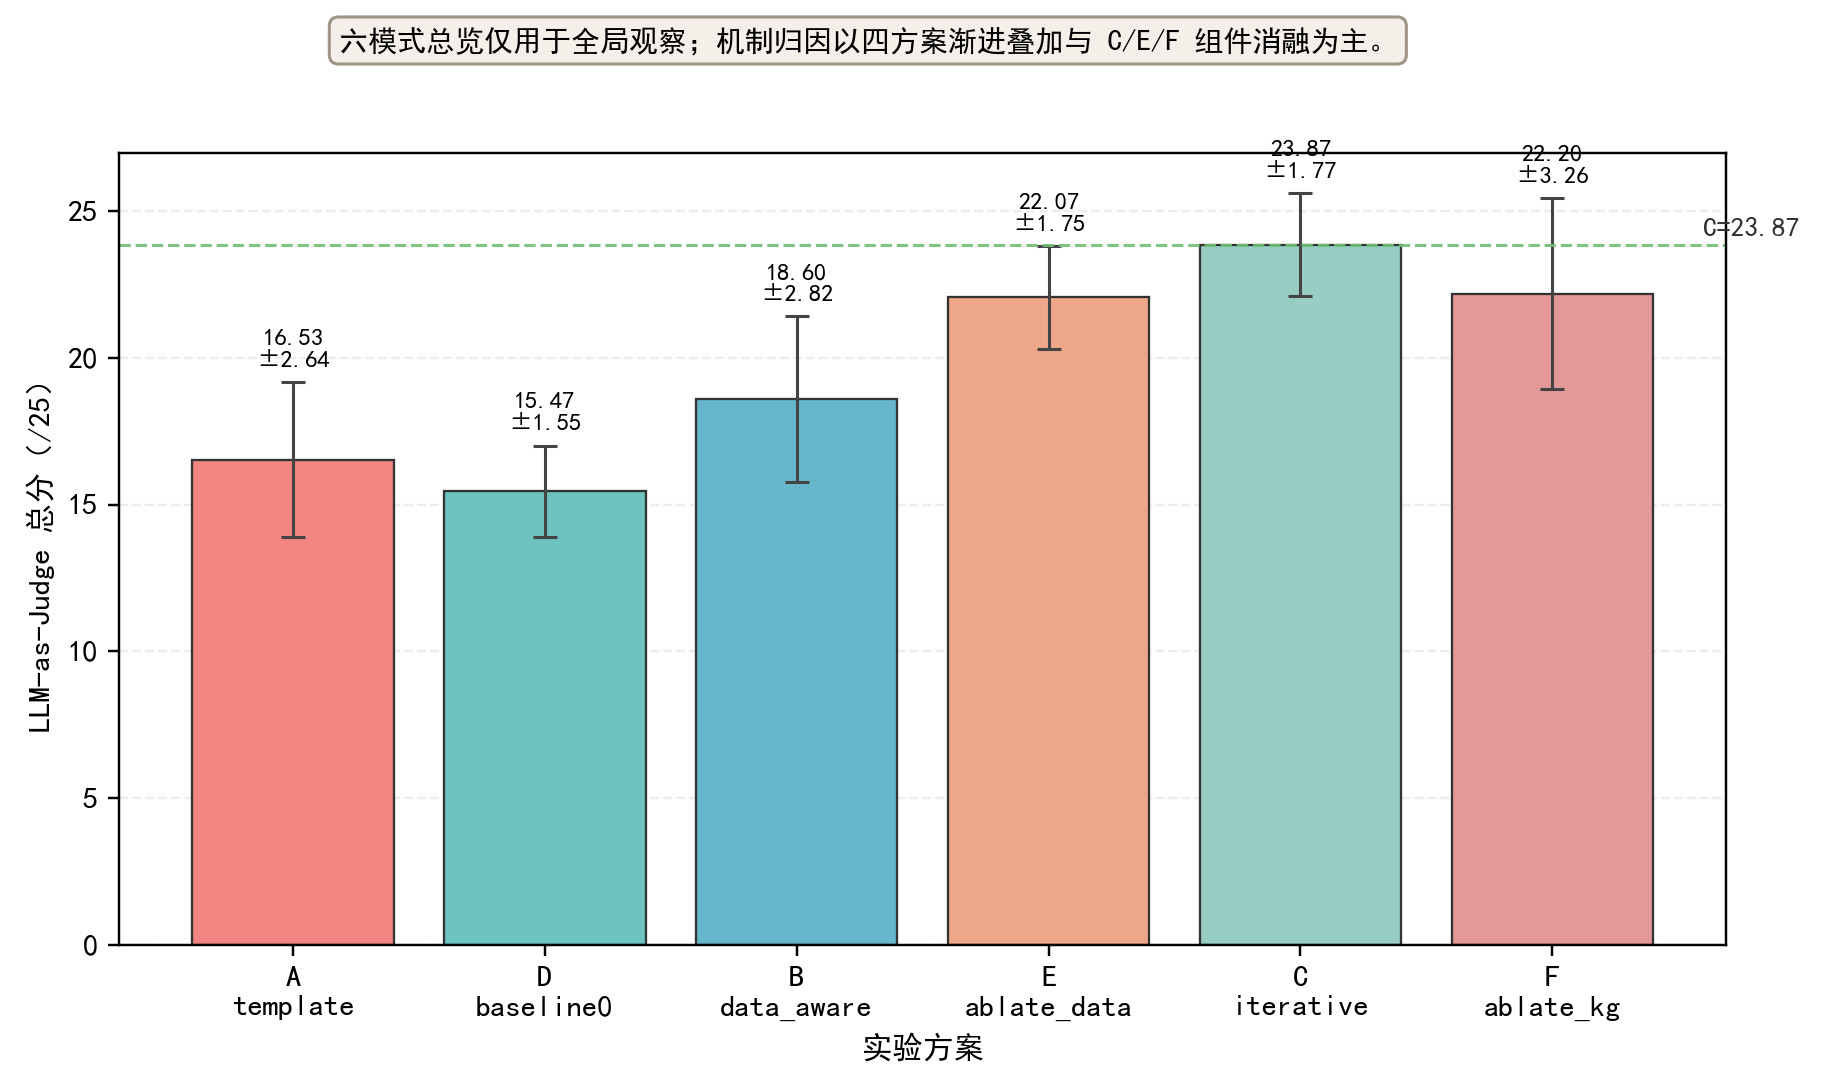
\includegraphics[width=0.78\textwidth]{figures/图5-2_六方案LLM总分柱状图.png}
\caption{六模式 LLM 总分总览（重复实验均值，误差线为标准差）}
\label{fig:ch5-overview}
\end{figure}

如图 \ref{fig:ch5-overview} 所示，六模式总览呈现出清晰分层：C\_iterative 的平均总分最高（23.87 $\pm$ 1.77），E\_ablate\_data 与 F\_ablate\_kg 处于第二梯队（分别为 22.07 $\pm$ 1.75 和 22.20 $\pm$ 3.26），B\_data\_aware 处于中间位置（18.60 $\pm$ 2.82），A\_template 与 D\_baseline0 则处于相对较低且彼此接近的区间（16.53 $\pm$ 2.64 和 15.47 $\pm$ 1.55）。这一总览说明完整系统在平均意义上最优，但六模式并列图本身只用于全局观察，不直接承担模块归因任务；系统为何变好以及各组件如何起作用，仍需回到渐进叠加和消融比较中分别解释。

\subsubsection{四方案渐进叠加主实验}

主实验关注 D\_baseline0、A\_template、B\_data\_aware 和 C\_iterative 四种模式。其核心目标不是给出单一排行榜，而是解释知识约束、数据感知与迭代优化如何逐步改变方案生成质量。

\begin{figure}[H]
\centering
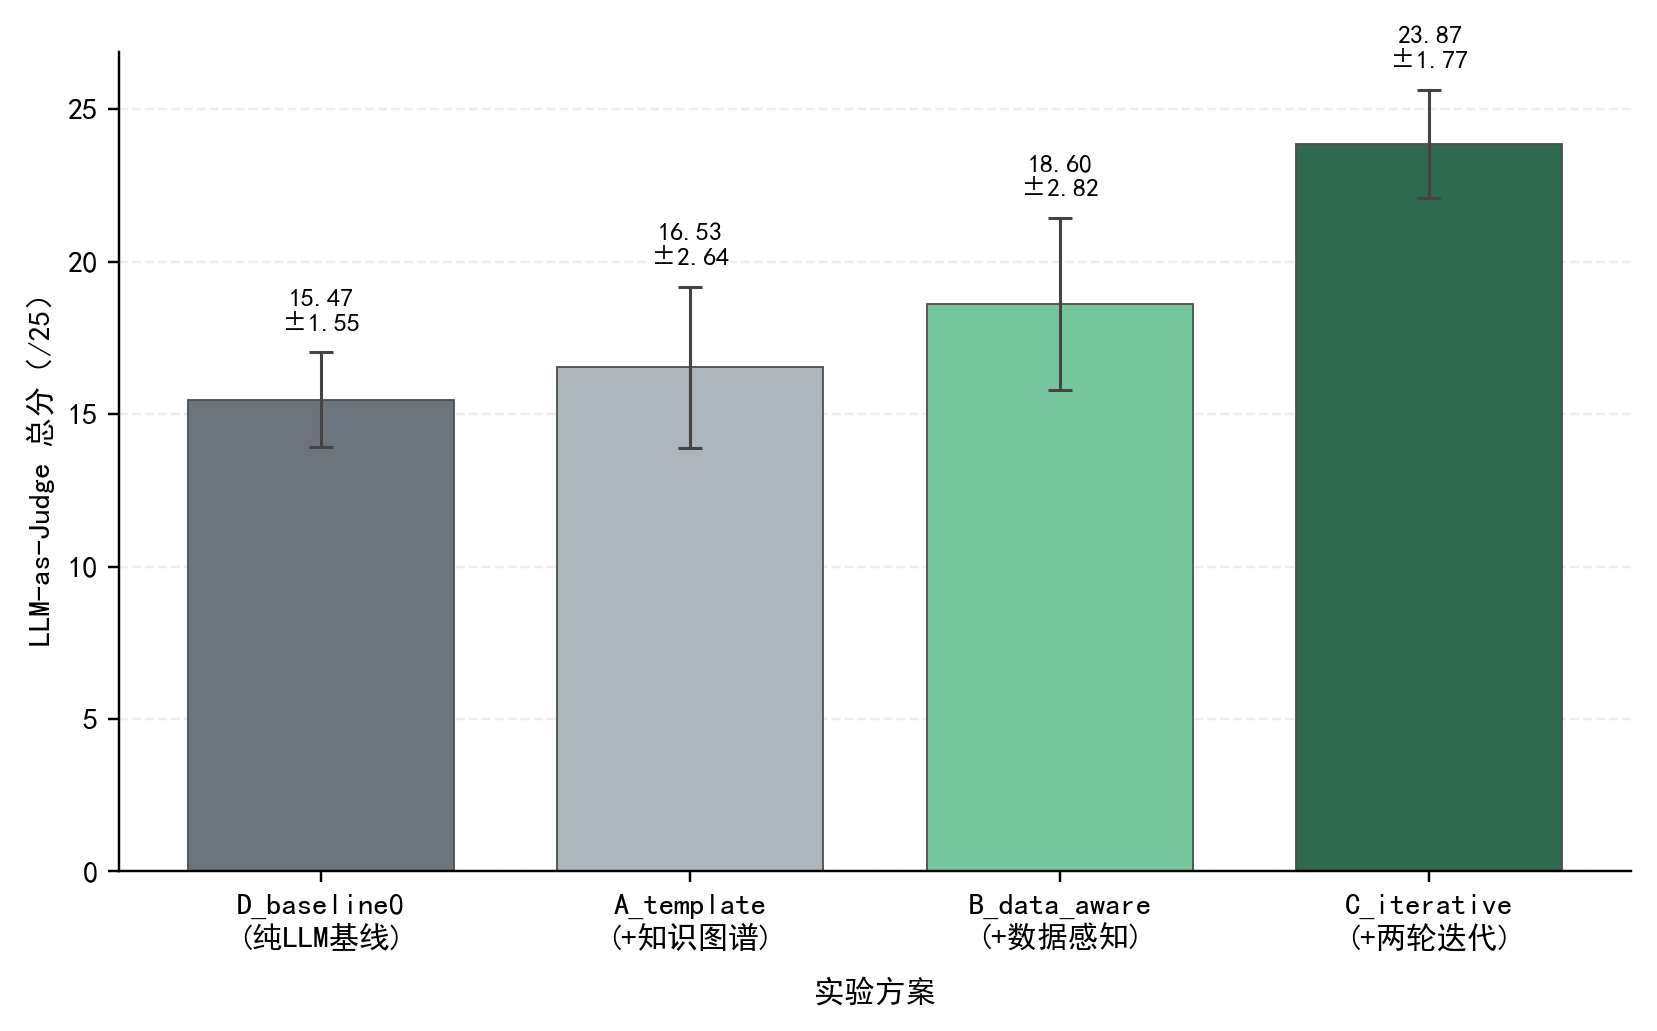
\includegraphics[width=0.72\textwidth]{figures/图5-1_四方案LLM总分柱状图.png}
\caption{四方案 LLM 总分对比（重复实验均值，误差线为标准差）}
\label{fig:ch5-main-total}
\end{figure}

\begin{table}[htbp]
\centering
\caption{四方案自动化指标对比（3 问题 $\times$ 5 次重复的均值 $\pm$ 标准差）}
\label{tab:main-auto}
\resizebox{\textwidth}{!}{
\begin{tabular}{lcccc}
\toprule
指标 & D\_baseline0 & A\_template & B\_data\_aware & C\_iterative \\
\midrule
数据列覆盖率 & 0.255 $\pm$ 0.051 & 0.276 $\pm$ 0.056 & 0.285 $\pm$ 0.053 & 0.358 $\pm$ 0.089 \\
方法多样性 & 2.667 $\pm$ 0.617 & 2.800 $\pm$ 0.561 & 2.667 $\pm$ 0.488 & 5.000 $\pm$ 0.655 \\
任务描述详细度 & 54.733 $\pm$ 20.518 & 55.627 $\pm$ 18.442 & 61.693 $\pm$ 18.554 & 85.167 $\pm$ 13.927 \\
针对性引用数 & 1.067 $\pm$ 1.100 & 1.200 $\pm$ 1.656 & 10.200 $\pm$ 4.161 & 14.200 $\pm$ 6.527 \\
控制变量数 & 1.733 $\pm$ 1.486 & 1.200 $\pm$ 1.207 & 0.400 $\pm$ 0.828 & 0.733 $\pm$ 0.961 \\
参数丰富度 & 6.333 $\pm$ 1.988 & 4.867 $\pm$ 1.552 & 5.133 $\pm$ 2.416 & 11.733 $\pm$ 3.240 \\
预期结论具体度 & 0.267 $\pm$ 0.320 & 0.300 $\pm$ 0.414 & 0.744 $\pm$ 0.288 & 0.427 $\pm$ 0.204 \\
数据洞察数量 & 0.000 $\pm$ 0.000 & 0.000 $\pm$ 0.000 & 2.800 $\pm$ 0.414 & 2.667 $\pm$ 0.816 \\
生成任务总数 & 2.800 $\pm$ 0.561 & 2.933 $\pm$ 0.458 & 2.800 $\pm$ 0.414 & 5.000 $\pm$ 0.655 \\
代码执行成功率 & 1.000 $\pm$ 0.000 & 1.000 $\pm$ 0.000 & 1.000 $\pm$ 0.000 & 1.000 $\pm$ 0.000 \\
\bottomrule
\end{tabular}
}
\vspace{0.3em}
\begin{minipage}{0.96\linewidth}
\footnotesize\raggedright
注：表中数值来自 3 个问题、每个问题 5 次重复实验的聚合结果；“控制变量数”受参数字段命名风格影响较大，仅作辅助观察。
\end{minipage}
\end{table}

\begin{table}[htbp]
\centering
\caption{四方案 LLM-as-Judge 评分对比（3 问题 $\times$ 5 次重复的均值 $\pm$ 标准差）}
\label{tab:main-llm}
\resizebox{\textwidth}{!}{
\begin{tabular}{lcccc}
\toprule
维度 & D\_baseline0 & A\_template & B\_data\_aware & C\_iterative \\
\midrule
相关性 & 3.73 $\pm$ 0.46 & 3.93 $\pm$ 0.46 & 4.07 $\pm$ 0.59 & 4.93 $\pm$ 0.26 \\
针对性 & 3.00 $\pm$ 0.00 & 3.40 $\pm$ 0.63 & 3.87 $\pm$ 0.83 & 4.73 $\pm$ 0.46 \\
方法合理性 & 3.27 $\pm$ 0.46 & 3.33 $\pm$ 0.62 & 3.40 $\pm$ 0.83 & 4.73 $\pm$ 0.46 \\
创新性 & 2.47 $\pm$ 0.52 & 3.20 $\pm$ 0.86 & 4.13 $\pm$ 0.52 & 4.73 $\pm$ 0.46 \\
深度 & 3.00 $\pm$ 0.54 & 2.67 $\pm$ 0.62 & 3.13 $\pm$ 0.74 & 4.73 $\pm$ 0.46 \\
总分(/25) & 15.47 $\pm$ 1.55 & 16.53 $\pm$ 2.64 & 18.60 $\pm$ 2.82 & 23.87 $\pm$ 1.77 \\
\bottomrule
\end{tabular}
}
\end{table}

\begin{figure}[H]
\centering
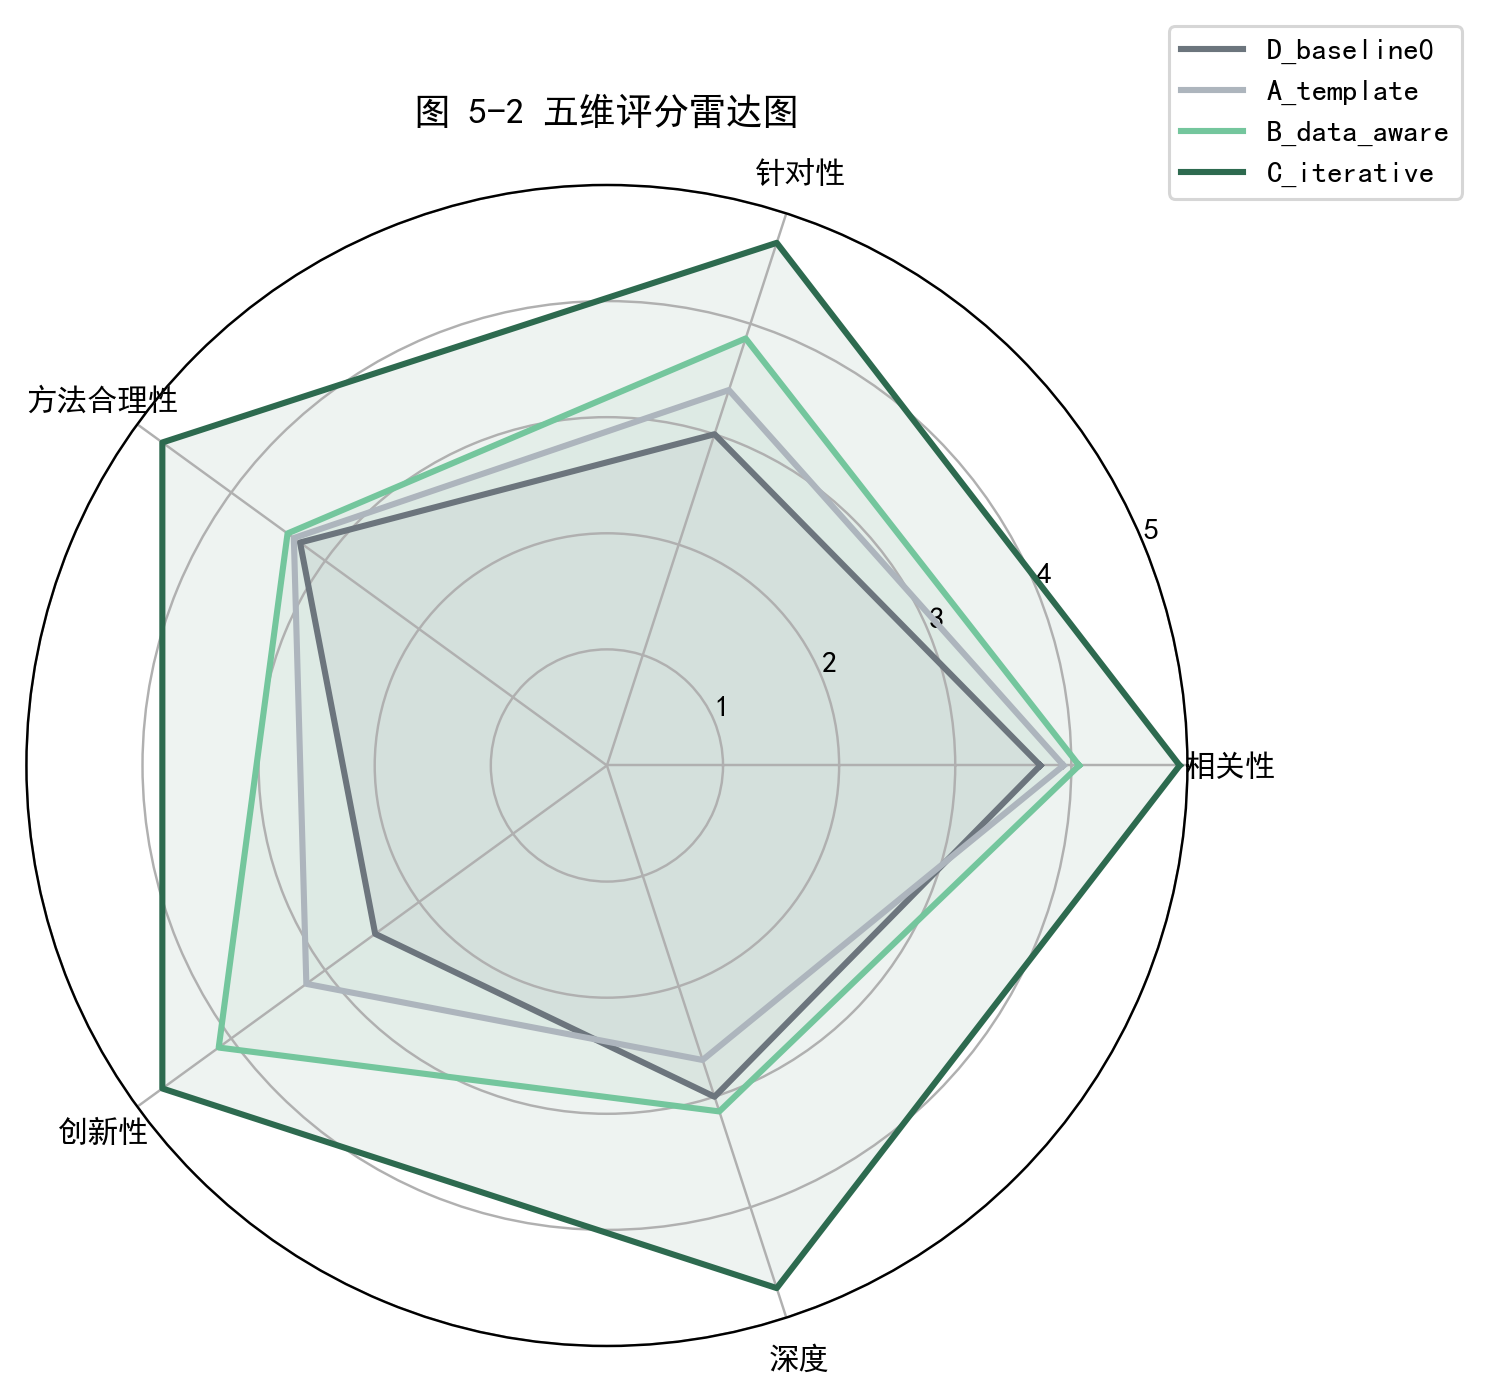
\includegraphics[width=0.68\textwidth]{figures/图5-2_五维评分雷达图.png}
\caption{四方案五维语义评分雷达图（重复实验均值）}
\label{fig:ch5-main-radar}
\end{figure}

\begin{figure}[H]
\centering
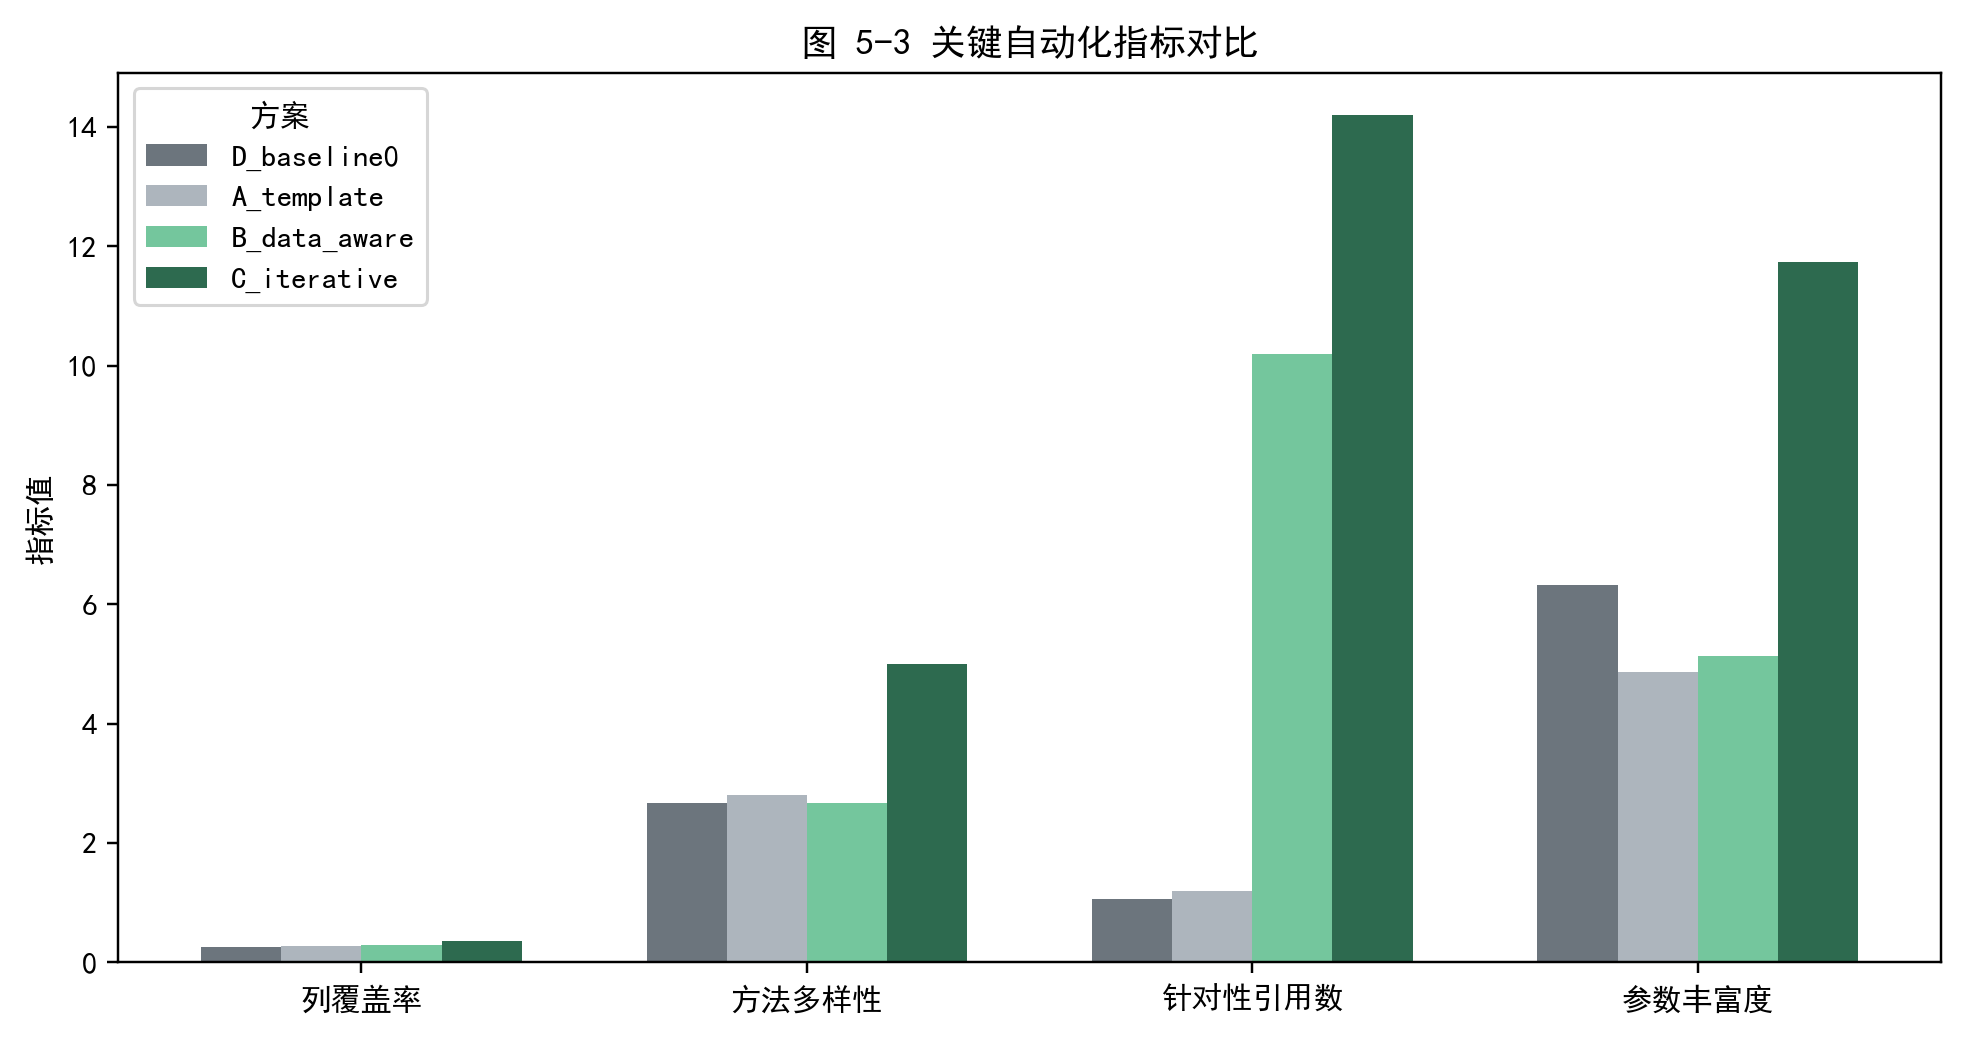
\includegraphics[width=0.84\textwidth]{figures/图5-3_自动化指标对比图.png}
\caption{四方案关键自动化指标对比（重复实验均值）}
\label{fig:ch5-main-auto}
\end{figure}

\begin{table}[htbp]
\centering
\caption{四方案问题级 LLM 总分明细（均值 $\pm$ 标准差）}
\label{tab:main-question}
\resizebox{\textwidth}{!}{
\begin{tabular}{lcccc}
\toprule
研究问题 & D\_baseline0 & A\_template & B\_data\_aware & C\_iterative \\
\midrule
Q1 技术影响力驱动因素 & 16.20 $\pm$ 2.05 & 17.00 $\pm$ 1.87 & 19.60 $\pm$ 1.95 & 22.20 $\pm$ 2.17 \\
Q2 技术融合趋势识别 & 15.20 $\pm$ 0.84 & 16.80 $\pm$ 4.03 & 17.40 $\pm$ 2.51 & 24.60 $\pm$ 0.89 \\
Q3 国家竞争态势评估 & 15.00 $\pm$ 1.58 & 15.80 $\pm$ 1.92 & 18.80 $\pm$ 3.83 & 24.80 $\pm$ 0.45 \\
\bottomrule
\end{tabular}
}
\end{table}

图 \ref{fig:ch5-main-total} 和表 \ref{tab:main-llm} 给出了主实验的核心结论。首先，C\_iterative 在四方案中显著领先，总分达到 23.87 $\pm$ 1.77，明显高于 B\_data\_aware 的 18.60 $\pm$ 2.82，也远高于 A\_template 与 D\_baseline0。其次，B\_data\_aware 稳定高于 A\_template 与 D\_baseline0，尤其在针对性、创新性和总分维度上体现出较清晰的领先。再次，A\_template 与 D\_baseline0 的均值差距相对有限：A 在相关性、针对性、方法合理性和创新性上略高于 D，但在深度维度仍低于 D，说明仅凭知识模板约束并不足以稳定拉开性能差距，其主要作用更接近“提供结构先验”而非“直接带来全面提升”。

自动化结构指标进一步解释了上述语义差异。表 \ref{tab:main-auto} 和图 \ref{fig:ch5-main-auto} 表明，完整模式 C 在列覆盖率、方法多样性、参数丰富度、任务总数和针对性引用数等关键指标上均处于显著领先位置，说明两轮迭代不仅增加了任务数量，更实质性地扩展了方法空间与证据引用密度。与单次实验版本不同，重复实验中的 B\_data\_aware 并未表现出“列覆盖率下降”的稳定特征，其列覆盖率均值（0.285）略高于 D\_baseline0（0.255），任务总数也基本相近（2.800 vs 2.800），但针对性引用数由 1.067 提升到 10.200。这说明数据感知在重复实验中表现出的主要效果不是“以广度换深度”，而是让系统在保持基础覆盖的同时更频繁地围绕真实数据证据组织任务。

从问题级结果看，三类研究问题对各增强模块的敏感性存在明显差异。Q2 中，C\_iterative 以 24.60 $\pm$ 0.89 显著领先其余三种模式，说明在同时需要整合图结构信号、文本语义与多步任务编排的结构—趋势类问题上，数据感知与迭代机制几乎是决定上限的必要条件。Q1 和 Q3 中，A 与 D 的差距均相对有限，而 B 和 C 的优势更加清晰，说明数据证据注入对开放问题的帮助更直接。总体上，主实验支持两个稳健判断：第一，数据感知是把系统从“纯语义规划”推进到“证据驱动规划”的关键机制；第二，两轮迭代是进一步把中等质量方案提升为高质量方案的核心环节。

\subsubsection{组件消融实验}

前述 D$\rightarrow$A$\rightarrow$B$\rightarrow$C 主实验解释了系统为何随着模块叠加而变好，但无法直接回答“在完整系统中，若单独移除某个组件，会造成多大影响”这一问题。为此，本文在 C\_iterative 的基础上设计了 E\_ablate\_data 和 F\_ablate\_kg 两组消融，用于分别考察数据感知和知识图谱的独立贡献。

\begin{table}[htbp]
\centering
\caption{组件消融自动化指标对比（3 问题 $\times$ 5 次重复的均值 $\pm$ 标准差）}
\label{tab:ablation-auto}
\resizebox{\textwidth}{!}{
\begin{tabular}{lccc}
\toprule
指标 & C\_iterative & E\_ablate\_data & F\_ablate\_kg \\
\midrule
数据列覆盖率 & 0.358 $\pm$ 0.089 & 0.349 $\pm$ 0.082 & 0.345 $\pm$ 0.062 \\
方法多样性 & 5.000 $\pm$ 0.655 & 4.533 $\pm$ 0.640 & 4.933 $\pm$ 0.961 \\
任务描述详细度 & 85.167 $\pm$ 13.927 & 83.853 $\pm$ 17.473 & 89.313 $\pm$ 28.003 \\
针对性引用数 & 14.200 $\pm$ 6.527 & 3.000 $\pm$ 2.752 & 14.533 $\pm$ 6.917 \\
参数丰富度 & 11.733 $\pm$ 3.240 & 11.467 $\pm$ 1.959 & 11.533 $\pm$ 2.642 \\
数据洞察数量 & 2.667 $\pm$ 0.816 & 0.000 $\pm$ 0.000 & 2.600 $\pm$ 1.056 \\
生成任务总数 & 5.000 $\pm$ 0.655 & 4.867 $\pm$ 0.516 & 4.867 $\pm$ 0.640 \\
代码执行成功率 & 1.000 $\pm$ 0.000 & 1.000 $\pm$ 0.000 & 1.000 $\pm$ 0.000 \\
\bottomrule
\end{tabular}
}
\end{table}

\begin{table}[htbp]
\centering
\caption{组件消融 LLM-as-Judge 评分对比（3 问题 $\times$ 5 次重复的均值 $\pm$ 标准差）}
\label{tab:ablation-llm}
\resizebox{\textwidth}{!}{
\begin{tabular}{lccc}
\toprule
维度 & C\_iterative & E\_ablate\_data & F\_ablate\_kg \\
\midrule
相关性 & 4.93 $\pm$ 0.26 & 4.73 $\pm$ 0.46 & 4.67 $\pm$ 0.62 \\
针对性 & 4.73 $\pm$ 0.46 & 4.33 $\pm$ 0.49 & 4.73 $\pm$ 0.59 \\
方法合理性 & 4.73 $\pm$ 0.46 & 4.53 $\pm$ 0.52 & 4.20 $\pm$ 0.68 \\
创新性 & 4.73 $\pm$ 0.46 & 3.87 $\pm$ 0.35 & 4.40 $\pm$ 0.91 \\
深度 & 4.73 $\pm$ 0.46 & 4.60 $\pm$ 0.51 & 4.20 $\pm$ 0.78 \\
总分(/25) & 23.87 $\pm$ 1.77 & 22.07 $\pm$ 1.75 & 22.20 $\pm$ 3.26 \\
\bottomrule
\end{tabular}
}
\end{table}

\begin{table}[htbp]
\centering
\caption{组件消融问题级 LLM 总分明细（均值 $\pm$ 标准差）}
\label{tab:ablation-question}
\resizebox{\textwidth}{!}{
\begin{tabular}{lccc}
\toprule
研究问题 & C\_iterative & E\_ablate\_data & F\_ablate\_kg \\
\midrule
Q1 技术影响力驱动因素 & 22.20 $\pm$ 2.17 & 21.20 $\pm$ 1.64 & 24.60 $\pm$ 0.89 \\
Q2 技术融合趋势识别 & 24.60 $\pm$ 0.89 & 22.40 $\pm$ 1.95 & 21.40 $\pm$ 1.52 \\
Q3 国家竞争态势评估 & 24.80 $\pm$ 0.45 & 22.60 $\pm$ 1.67 & 20.60 $\pm$ 4.78 \\
\bottomrule
\end{tabular}
}
\end{table}

从平均结果看，C\_iterative 在消融比较中仍保持最高总分（23.87 $\pm$ 1.77），高于 E\_ablate\_data 的 22.07 $\pm$ 1.75 和 F\_ablate\_kg 的 22.20 $\pm$ 3.26。这一结果与单次实验版本中“移除知识图谱后总体更好”的观察不同，表明在重复实验口径下，完整系统的平均优势是可以复现的。

对比 C 与 E，可以较清晰地观察到数据感知模块的直接贡献。表 \ref{tab:ablation-auto} 显示，移除数据感知后，针对性引用数由 14.200 大幅降至 3.000，数据洞察数量由 2.667 变为 0，方法多样性和任务总数也同步下降；表 \ref{tab:ablation-llm} 则显示，E 在针对性、创新性和总分上均低于 C。说明 DataPreview 和 GraphPreview 并非仅增加上下文长度，而是实质改变了任务设计的出发点，使系统能够围绕当前数据中已经显露的模式组织分析路径。

对比 C 与 F，可以更细致地理解知识图谱的任务依赖性。平均结果上，F 的总分低于 C，说明知识图谱在整体上仍提供了正向作用；但表 \ref{tab:ablation-question} 同时表明，这一收益并不均匀。Q1 中，F 以 24.60 $\pm$ 0.89 高于 C 的 22.20 $\pm$ 2.17，说明在开放度更高、可由数据直接驱动多种解释路径的问题上，移除静态图谱约束可能释放更多探索空间。相反，Q2 和 Q3 中，C 分别以 24.60 $\pm$ 0.89 和 24.80 $\pm$ 0.45 明显高于 F 的 21.40 $\pm$ 1.52 和 20.60 $\pm$ 4.78，说明当问题具有较清晰的结构锚点、需要多步链式分析时，知识图谱能够更稳定地约束变量选择与方法路径，从而提升方案质量。

综合主实验与消融实验可以得到如下机制解释：数据感知回答“当前数据最值得看什么”，知识图谱回答“面对这类证据通常该怎么分析”，两轮迭代则负责“发现第一轮不足后如何继续深化”。三者共同组成了完整系统的性能来源。若只保留其中任意两个组件，系统仍可得到较高分数；但若要在多种问题上同时保持高针对性、高方法合理性和高深度，完整配置仍然最稳。

\subsubsection{有效性威胁与缓解}

第一，\textbf{统计显著性仍待补充}。本文已经对 6 种模式、3 个问题各独立重复运行 5 次，显著降低了单次观察带来的偶然性风险，但尚未进一步对关键差异进行正式显著性检验。因此，当前结论可被视为“具有重复证据支持的稳健趋势”，后续仍需通过 bootstrap 置信区间、Friedman 检验或 Wilcoxon 符号秩检验补充统计推断。

第二，\textbf{评估主体单一}。LLM-as-Judge 虽采用匿名并列评分和低温度参数缓解偏差，但仍可能偏好某些表述风格、方法路径或文本长度。本文通过在同一“问题 × 重复轮次”内混排六种方案降低标签干扰，但从方法论上看，后续仍应加入人工专家盲审或多模型集成评分作为交叉校验。

第三，\textbf{问题集规模有限}。当前仅覆盖三个研究问题，虽分别代表解释型、结构—趋势型和比较评估型任务，但在统计外推和任务多样性方面仍然有限。后续需扩展问题库并在更多数据集上复验关键结论，以提高外部有效性。

第四，\textbf{实现配置依赖}。本文控制了统一模型版本、提示模板和执行环境，使相对比较更具可比性，但不同模型、不同提示配置和不同计算环境下是否仍保持类似排序，仍需后续补充验证。

\subsection{本章小结}

本章采用“六模式总览 + 四方案渐进叠加主实验 + 组件消融”的组织方式，对 90 组重复实验结果进行了系统分析。总体来看，C\_iterative 是当前最优且最稳定的配置；B\_data\_aware 稳定优于 A\_template 与 D\_baseline0，说明数据感知是推动方案从语义驱动走向证据驱动的关键机制；知识图谱在平均意义上提供正向贡献，但收益强度具有明显任务依赖性。与单次实验相比，重复实验使本文的结论从“初始观察”转化为“具有重复支持的机制判断”，为后续应用示例与总结章节提供了更稳健的实证基础。


\section{系统应用示例}

\subsection{应用场景与使用角色}

本系统在实际应用中主要对应三类用户角色。第一类是专利计量研究者，关注分析流程的可复现性、变量定义的可解释性以及统计结论的可验证性。第二类是技术情报分析师，关注快速形成多视角研判并输出可执行洞察。第三类是企业知识产权管理者，关注高价值技术布局识别、竞争风险监测与专利资产配置。

与传统手工流程相比，系统将"问题理解$\rightarrow$方案设计$\rightarrow$代码执行$\rightarrow$结果解释"串联为自动化闭环，尤其在规划阶段引入数据证据，降低了人工试错成本。对上述三类角色而言，系统的核心价值不是替代领域判断，而是提供稳定、可追踪、可复核的分析底座。

为展示系统在不同分析场景下的应用方式与输出形态，本章选取三个研究问题作为应用案例，分别对应因果驱动分析、技术融合趋势识别和国家竞争态势评估三类典型专利计量任务。三者共同覆盖“机制解释”“结构趋势识别”“竞争比较评估”三种常见研究目标，因此可作为系统能力展示的说明性案例集。三个案例均采用完整系统（C\_iterative 模式），所有数据来自实际实验产出文件。

需要说明的是，本章定位为\textbf{流程展示与中间产物说明}，重点回答“系统如何把研究问题转化为分步任务、代码和结果解释”；其作用是补充展示第五章定量实验背后的执行链路，而非提供独立于第五章之外的新一轮效果验证。因此，本章中的案例结果应被理解为完整系统在三个代表性问题上的样例输出，系统优劣的统一判断仍以第五章的对比实验为准。

\subsection{案例一：技术影响力驱动因素分析}

本案例选择 Q1"分析数据安全领域的技术影响力驱动因素"，展示从输入目标到输出报告的两轮完整分析过程\footnote{本案例数据来源为系统实验产出文件 \texttt{experiment\_q1\_C\_iterative.json}。}。

\subsubsection{输入与数据感知}

用户输入研究问题后，系统解析目标类型和数据边界。研究目标为"分析数据安全领域的技术影响力驱动因素"，目标类型为因果/驱动因素识别，数据集为 \texttt{data/new\_data.XLSX}，包含 10,000 条数据安全领域专利、22 个字段。

Strategist 调用 DataPreview 与 GraphPreview，生成 3 条被选中用于蓝图规划的洞察：

\textbf{洞察 I1}（statistical）：近年授权专利被引量骤降——反映技术迭代加速，需在分析中控制专利年龄，否则会混淆真实影响力。

\textbf{洞察 I2}（graph\_structural）：H04L9/40 为核心枢纽——可限定分析范围至该 IPC 主导的子网络，提升假设检验的针对性。

\textbf{洞察 I3}（statistical）：法律状态复杂性提升引用活跃度——提示需控制法律状态以隔离商业化干扰。

\subsubsection{第一轮分析：探索性验证}

基于洞察和双知识图谱，Strategist 生成第一轮 DAG 蓝图，包含 2 个分析任务：

\textbf{任务 1：变量计算（variable\_calculation）}

% 请确保导言区包含：\usepackage{booktabs, array}

\begin{table}[htbp]
\centering
\caption{案例一第一轮任务1配置}
\label{tab:case1-r1-t1}
\begin{tabular}{>{\centering\arraybackslash}p{3.2cm} >{\raggedright\arraybackslash}p{10.4cm}}
\toprule % 顶线
项目 & 内容 \\
\midrule % 栏目线
研究问题 & 如何计算每项专利的技术多样性并标准化其影响力以排除时间偏差？ \\
使用列   & IPC分类号、被引用专利数量、授权日 \\
参数     & reference\_year=2026 \\
\bottomrule % 底线
\end{tabular}
\end{table}

执行结果：有效专利 9,879 条，技术多样性均值为 3.89（中位数 3.0，标准差 2.88，范围 1-78），呈明显右偏分布。以 2026 年 1 月为基准时点，平均专利年龄为 2.7 年，标准化被引量均值为 0.57，有效消除了专利年龄带来的时间累积效应，与洞察 I1 的判断一致。

\textbf{任务 2：假设检验（hypothesis\_test）}

% 请确保在 LaTeX 文档的导言区添加：
% \usepackage{booktabs, array}

\begin{table}[htbp]
\centering
\caption{案例一第一轮任务2配置}
\label{tab:case1-r1-t2}
\begin{tabular}{>{\centering\arraybackslash}p{3.2cm} >{\raggedright\arraybackslash}p{10.4cm}}
\toprule % 顶线（粗线）
项目 & 内容 \\
\midrule % 栏目线（细线）
研究问题 & 技术跨界度对技术影响力是否有负向影响？ \\ \addlinespace[0.5ex] % 增加一点行间距，防止文字拥挤
使用列   & IPC分类号、被引用专利数量、授权日、法律状态/事件、IPC主分类号 \\ \addlinespace[0.5ex]
控制变量 & patent\_age, legal\_status\_dummies \\
\bottomrule % 底线（粗线）
\end{tabular}
\end{table}

执行结果：假设未获支持。全样本回归中技术多样性系数不显著（$\beta$=0.006, p=0.909, R²=0.066, n=10,000）；在 H04L9/40 子群中系数方向为负但同样不显著（$\beta$=-0.157, p=0.147, R²=0.039, n=816）。该"零结果"否定了"技术融合必然损害影响力"的假设，为第二轮提供了明确的探索方向。

\subsubsection{第二轮分析：差距修补与深化验证}

系统读取第一轮结果后，自动进行差距分析：第一轮排除了技术跨界度作为显著驱动因素的假设，但洞察中提及的法律状态因果关系、H04L9/40 共现强度影响、高连接度发明人等方向未被检验。系统据此在第二轮引入控制变量（授权年份、IPC 主分类号前 4 位）、交互项（法律状态×IPC 核心度）及非线性建模（负二项回归）。

第二轮 DAG 蓝图包含 2 个深化任务：

\textbf{任务 R2\_1：IPC 共现网络特征工程 + 负二项回归}

% 请确保导言区已添加：\usepackage{booktabs, array}

\begin{table}[htbp]
\centering
\caption{案例一第二轮任务R2\_1配置}
\label{tab:case1-r2-t1}
\begin{tabular}{>{\centering\arraybackslash}p{3.2cm} >{\raggedright\arraybackslash}p{10.4cm}}
\toprule % 顶线
项目 & 内容 \\
\midrule % 栏目线
研究问题 & IPC 共现网络中 H04L9/40 的共现强度是否显著正向预测专利被引量？ \\ \addlinespace[0.5ex]
方法     & 负二项回归（替代 OLS，适应计数数据） \\ \addlinespace[0.5ex]
控制变量 & 授权年份固定效应, IPC 主分类前缀 \\
\bottomrule % 底线
\end{tabular}
\end{table}

该任务将 GraphPreview 的 IPC 共现网络信息转化为回归自变量，实现"图特征$\rightarrow$统计建模"路径。

\textbf{任务 R2\_2：发明人网络分析 + 文本挖掘 + 中介检验}

% 请确保在导言区添加：\usepackage{booktabs, array}

\begin{table}[htbp]
\centering
\caption{案例一第二轮任务R2\_2配置}
\label{tab:case1-r2-t2}
\begin{tabular}{>{\centering\arraybackslash}p{3.2cm} >{\raggedright\arraybackslash}p{10.4cm}}
\toprule % 顶线
项目 & 内容 \\
\midrule % 栏目线
研究问题 & 高连接度发明人所参与的专利是否更倾向于包含特定技术主题，且该主题是否中介其对被引量的正向影响？ \\ \addlinespace[0.5ex]
方法     & BERT 主题建模 + 负二项回归 + 中介效应检验 \\ \addlinespace[0.5ex]
参数     & high\_degree\_threshold=30 \\
\bottomrule % 底线
\end{tabular}
\end{table}

该任务同时利用发明人合作网络和摘要内容，实现"网络位置$\rightarrow$技术主题$\rightarrow$影响力"的跨层级机制检验。

两轮合计产出 4 个分析任务，全部执行成功。分析层次从第一轮的"效应是否存在"提升至第二轮的"效应的机制、路径和边界条件"。

\subsection{案例二：技术融合趋势识别}

本案例选择 Q2"识别数据安全领域的技术融合趋势"，重点展示系统对图结构信息和文本内容的综合利用能力\footnote{本案例数据来源为系统实验产出文件 \texttt{experiment\_q2\_C\_iterative.json}。}。

\subsubsection{数据感知与洞察选择}

系统为本问题选中 3 条核心洞察：

\textbf{洞察 I1}（graph\_structural）：H04L9/40 在 IPC 共现网络中度数高达 904，是技术融合网络的核心枢纽，可作为融合分析的锚点。

\textbf{洞察 I2}（statistical）：质押状态专利平均被引 84.08 次，远高于普通授权专利的 11.19 次，提示高融合度专利具有更高商业价值。

\textbf{洞察 I3}（content\_driven）：摘要中频繁出现"安全组件嵌入"、"SoC 测试密钥"等硬件级安全术语，结合 IPC 分布跨越 A、F、G 等部类，提示硬件级安全机制成为跨领域融合新焦点。

\subsubsection{第一轮分析：融合结构探索}

第一轮 DAG 蓝图包含 3 个任务，分别从网络结构、法律状态关联和时间趋势三个角度探索融合特征：

\textbf{任务 1：H04L9/40 桥接 IPC 提取（variable\_calculation）}。从 IPC 共现网络中提取 H04L9/40 子图，识别直接连接的 IPC 编码并按部类聚合，计算跨部类边占比。结果显示 H04L9/40 子图中跨部类边占比达 78.3\%，Top 3 桥接分类为 G16H50/70（医疗 AI）、A61B5/00（医疗设备）和 B61L27/00（铁路控制），表明安全协议已深度渗透至医疗和交通领域。

\textbf{任务 2：法律状态与 IPC 多样性关联检验（hypothesis\_test）}。按法律状态分组计算 IPC Shannon 熵和跨部类引用比例，进行独立样本 t 检验。结果显示质押专利 IPC Shannon 熵为 2.91，显著高于普通授权专利的 2.43（p<0.01，效应量 d=0.42），跨部类引用比例高出 31\%，提示技术融合度与商业价值之间存在显著相关性。

\textbf{任务 3：硬件级安全专利时间趋势（variable\_calculation）}。使用 BERT 模型对摘要进行安全层级分类（硬件/固件/软件），按年度聚合。结果显示，硬件安全专利占比由 2023 年的 18.2\% 提升至截至 2026 年 1 月样本的 34.7\%。由于 2026 年仅覆盖截至 1 月的最新观测点，本文不将其解释为完整年度增速，而仅比较同口径下的阶段性升幅；按该口径，硬件层的上升幅度仍高于固件层（+9.3\%）和软件层（-5.2\%），说明硬件级安全议题持续升温。

\subsubsection{第二轮分析：融合机制深化}

系统识别第一轮的差距：未对 H04L9/40 共现专利进行语义层面的主题建模，未量化硬件安全关键词在各 IPC 部类的渗透强度差异，法律状态对引用的影响未控制 IPC 多样性作为混杂变量。第二轮生成 3 个深化任务：

\textbf{任务 R2\_1：层次回归分析}。在控制 IPC 分类多样性和技术子域固定效应后，质押专利仍显示额外 62.3 次引用增量（p<0.001），权利转移状态额外增加 18.7 次（p=0.003），证实法律状态复杂性独立于技术广度对引用深度的正向影响。

\textbf{任务 R2\_2：跨领域硬件安全术语提取}。使用预训练中文 BERT 提取摘要中的硬件安全术语，按 IPC 部类分组计算年度关键词密度。结果显示，A/F/G/H 部类的硬件安全关键词密度持续上升，截至 2026 年 1 月的最新观测点仍明显高于其他部类。按同一阶段口径估算，A/F/G/H 部类关键词密度增幅为 37.2\%，高于其他部类的 8.1\%；其中 A 部（医疗）和 F 部（机械）增幅最突出，分别为 52.4\% 和 48.7\%。

\textbf{任务 R2\_3：IPC-摘要联合主题建模}。对含 H04L9/40 的专利进行 LDA 主题建模（K=8），结合共现 IPC 标注语义。识别出 5 个显著融合簇：5G+医疗（28.3\%）、车联网认证（22.1\%）、工业物联网安全（19.7\%）、区块链身份（15.4\%）和消费电子可信执行环境（14.5\%）。

两轮合计产出 6 个分析任务，全部执行成功。系统从宏观融合结构（跨部类边占比）逐步深入到微观融合簇识别（5 个具体场景），体现了两轮迭代从"现象发现"到"机制解释"的分析深化路径。

\subsection{案例三：国家竞争态势评估}

本案例选择 Q3"评估不同国家/地区在数据安全领域的竞争态势"，重点展示系统在比较分析和多维指标构建场景下的能力\footnote{本案例数据来源为系统实验产出文件 \texttt{experiment\_q3\_C\_iterative.json}。}。

\subsubsection{数据感知与洞察选择}

系统为本问题选中 3 条核心洞察：

\textbf{洞察 I1}（statistical）：质押专利被引量异常显著（84.08 vs 11.19），可作为"高价值专利"的量化标识，避免仅依赖数量指标评估竞争力。

\textbf{洞察 I2}（graph\_structural）：美国在优先权合作网络中占据核心位置（度数=14），反映其在全球技术部署中的枢纽地位。

\textbf{洞察 I3}（graph\_structural）：H04L9/40 作为核心技术锚点，可聚焦分析各国在该协议上的布局差异，避免泛化的"数据安全"讨论。

\subsubsection{第一轮分析：竞争格局探索}

第一轮 DAG 蓝图包含 3 个任务：

\textbf{任务 1：质押专利与网络中心性关联检验（hypothesis\_test）}。按法律状态分组计算平均入度（被引次数），进行双样本 t 检验。质押专利平均被引 84.08 次，显著高于普通授权专利的 11.19 次（Cohen's d=0.67，p<0.00001），支持将质押状态视为高价值专利的候选标识。

\textbf{任务 2：国家网络中心性与产出质量回归分析（regression）}。构建优先权国家合作网络，计算各国度中心性，与专利族规模和引用影响力进行回归分析。国家度中心性对族规模和引用影响力呈中等正向效应（$\beta$=0.42，p=0.001，R²=0.31），美国（度数=14）在技术产出数量和全球控制力上均显著领先。

\textbf{任务 3：H04L9/40 核心协议的国家分布分析（data\_summary）}。按优先权国家对 H04L9/40 主分类专利进行分组统计。美国占 38\%（平均 4.2 次引用），侧重"动态证书生成"；中国占 25\%（平均 2.1 次引用），侧重"端到端加密"；韩国占 12\%，侧重"5G 用户面安全"。各国在核心协议上呈现差异化技术路线。

\subsubsection{第二轮分析：竞争机制深化}

系统识别第一轮的差距：未系统整合国家、技术、价值三维关系，未对 H04L9/40 内部子领域进行国家级主题聚类，质押专利的高引用行为未控制专利年龄的混杂影响。第二轮生成 2 个深化任务：

\textbf{任务 R2\_1：国家-技术子类聚类与优势分析}。对含 H04L9/40 的专利提取剩余 IPC 编码和摘要文本，进行主题聚类，计算各簇的国家分布 Shannon 熵和主导国家占比，识别各国技术优势领域。

\textbf{任务 R2\_2：高价值专利国家归属与年龄控制引用分析}。提取质押状态样本标注优先权国家，计算专利年龄（2026 - 授权年），使用协方差分析（ANCOVA）以被引量为因变量、法律状态为因素、专利年龄为协变量，检验质押组的引用优势是否独立于年龄效应，并报告质押专利国家 Top 5 分布。

两轮合计产出 5 个分析任务，全部执行成功。系统从第一轮的宏观竞争格局描述（国家数量对比、中心性排名）深化至第二轮的微观竞争机制解释（子领域优势识别、年龄控制后的独立效应验证）。

\subsection{三案例综合评价}

\subsubsection{执行统计对比}

% 请确保在导言区添加：\usepackage{booktabs, array}

\begin{table}[htbp]
\centering
\caption{三案例执行统计对比}
\label{tab:case-comparison}
\resizebox{\textwidth}{!}{
\begin{tabular}{>{\centering\arraybackslash}p{2.3cm} >{\raggedright\arraybackslash}p{3.8cm} >{\raggedright\arraybackslash}p{3.8cm} >{\raggedright\arraybackslash}p{3.8cm}}
\toprule % 顶线
维度 & Q1 影响力驱动因素 & Q2 技术融合趋势 & Q3 国家竞争态势 \\
\midrule % 栏目线
第一轮任务数 & 2 & 3 & 3 \\
第二轮任务数 & 2 & 3 & 2 \\
任务总数     & 4 & 6 & 5 \\
执行成功率   & 100\% & 100\% & 100\% \\ \addlinespace[0.5ex]
分析类型覆盖 & 回归、中介检验 & 图分析、主题建模、层次回归 & 网络分析、ANCOVA、聚类 \\
\bottomrule % 底线
\end{tabular}
}
\end{table}

三个案例在任务结构上存在显著差异：Q1 偏因果识别，任务链为"变量构建$\rightarrow$假设检验$\rightarrow$机制验证"；Q2 偏结构与趋势，任务链为"网络提取$\rightarrow$关联检验$\rightarrow$主题聚类"；Q3 偏比较与评估，任务链为"指标构建$\rightarrow$国家对比$\rightarrow$优势归因"。这一差异与系统"共框架、异任务"的设计目标相符——同一架构能够根据研究问题自动生成差异化的分析路径。

\subsubsection{两轮迭代效果对比}

% 请确保导言区已添加：\usepackage{booktabs, array}

\begin{table}[htbp]
\centering
\caption{两轮迭代效果对比}
\label{tab:iteration-comparison}
\resizebox{\textwidth}{!}{
\begin{tabular}{>{\centering\arraybackslash}p{2.3cm} >{\raggedright\arraybackslash}p{5.7cm} >{\raggedright\arraybackslash}p{5.7cm}}
\toprule % 顶线
维度 & 第一轮共性特征 & 第二轮共性特征 \\
\midrule % 栏目线
分析层次     & 效应存在性检验 & 机制、路径与边界条件 \\ \addlinespace[0.5ex]
典型方法     & OLS 回归、t 检验、描述统计 & 负二项回归、层次回归、ANCOVA、主题建模 \\ \addlinespace[0.5ex]
数据源       & 结构化字段 & 结构化字段 + 图特征 + 文本内容 \\ \addlinespace[0.5ex]
控制变量     & 少量（1-2 个） & 多层次（年龄、固定效应、交互项） \\ \addlinespace[0.5ex]
典型深化模式 & — & 非线性替代、混杂控制、跨层级机制检验 \\
\bottomrule % 底线
\end{tabular}
}
\end{table}

三个案例均展现了从第一轮到第二轮的一致性深化模式：第一轮建立基础变量关系并发现初步信号（包括零结果），第二轮基于差距分析引入更严格的统计控制、更丰富的数据源和更深层的机制检验。该模式表明两轮迭代机制在这三类分析场景下具有较好的适用性。

\subsubsection{应用效果总结}

基于三个案例，可总结三方面应用效果：

第一，方案可解释性。每个任务均可追溯至洞察条目和图谱路径。例如 Q1 任务 1 的"标准化被引量消除时间偏差"源于洞察 I1，Q1 任务 2 的"控制法律状态"源于洞察 I3，Q2 任务 1 的"H04L9/40 子图提取"源于洞察 I1，Q3 任务 2 的"国家度中心性"源于洞察 I2。这种"洞察$\rightarrow$任务$\rightarrow$结论"的证据链避免了黑箱式自动分析。

第二，执行可复核性。三个案例共 15 个任务全部执行成功，蓝图 JSON、技术规格、Python 代码和执行结果均有落盘文件，可复跑、可对比、可审计。

第三，迭代驱动深化。三个案例均展现了"第一轮发现$\rightarrow$差距识别$\rightarrow$第二轮深化"的自适应模式。Q1 从"零结果"转向替代机制探索，Q2 从宏观融合结构深入到 5 个具体融合簇，Q3 从国家数量对比深化至年龄控制后的独立效应验证。这些案例共同表明两轮迭代机制能够根据第一轮的实际结果自适应地调整分析方向，而非简单重复或放大初始假设。

\subsection{本章小结}

本章通过三个完整案例（技术影响力驱动因素分析、技术融合趋势识别、国家竞争态势评估）展示了系统从“研究问题输入”到“洞察生成—任务规划—代码执行—结果解释”的端到端应用流程。三个案例覆盖因果分析、趋势识别和比较评估三类典型专利计量任务，共产出 15 个分析任务且全部执行成功，说明在当前实现下，数据感知机制和两轮迭代机制已经能够在不同场景中稳定地生成可执行、可追溯的分析工作流。案例同时表明，系统并非简单替代研究者的领域判断，而是以“洞察—任务—证据链”的形式提供结构化决策支持，降低了手工试错成本、提高了方案与数据之间的一致性。需要强调的是，本章侧重展示执行链路和输出形态，本身不构成对系统效果的独立评估；关于各模块的相对贡献及总体优劣，仍应结合第五章的对比实验结果以及后续可能的重复实验一并加以判断。

\section{总结与展望}

\subsection{研究结论}

本文围绕“数据感知的多智能体专利分析方案自动生成”开展研究，完成了问题定义、系统设计、工程实现与实验验证四项工作。

在问题层面，本文指出现有大语言模型自动化分析系统的主要短板不在执行阶段，而在规划阶段：系统能够完成代码生成与执行，但未必能够在给定具体数据集时设计出与数据事实相匹配的高质量分析方案。该问题在专利计量场景中尤为突出，因为任务不仅要求结果产出，更要求变量解释、方法匹配与结论可复核。

在方法层面，本文提出“数据感知前置 + 双知识图谱协同 + 两轮迭代优化”的整体框架：先由 DataPreview 和 GraphPreview 提取可操作证据，再利用因果图谱与方法图谱组织假设空间和方法空间，最后通过执行反馈驱动第二轮验证性深化，从而把一次性分析升级为可追溯的探索—验证闭环。

在工程层面，本文实现了基于工作流编排框架的四智能体系统，并完成从输入研究问题到输出分析报告的端到端闭环，形成可复跑、可追踪、可审计的实验资产。

在实证层面，本文采用“主实验渐进叠加 + 组件消融 + 重复实验”的组织方式，对 6 种模式、3 个问题各重复运行 5 次，共完成 90 组实验。重复实验结果表明，完整方案 C\_iterative 在六模式总览中保持最高平均总分（23.87/25），且在相关性、针对性、方法合理性、创新性和深度五个维度上均表现稳定。结合实验结果，可以形成以下四项具体结论：

第一，数据感知是提升方案质量的稳定关键。与 A 和 D 相比，数据感知模式 B 在重复实验中稳定取得更高的语义评分和更强的数据证据引用，说明在规划前显式引入数据分布、图结构与样本语义证据，能够有效推动方案从“问题语义驱动”转向“数据证据驱动”。

第二，两轮迭代是拉开系统上限的核心机制。C\_iterative 在主实验四模式中显著高于其他方案，不仅总分最高，而且在方法多样性、参数丰富度、任务数和五维语义评分上均呈现更均衡的领先，说明第二轮并非简单重复第一轮，而是围绕证据缺口进行补证据、换方法和做稳健性分析。

第三，知识图谱具有正向但任务依赖的贡献。组件消融结果显示，移除知识图谱后总体平均表现由 C 的 23.87 降至 F 的 22.20，说明知识图谱在平均意义上仍提供正向增益；但分问题结果同时表明，图谱收益并不均匀，在结构锚点清晰、分析链条较长的问题上更明显，在开放度更高的问题上则需要与数据证据更紧密协同，避免静态路径过度约束。

第四，系统已表现出较好的工程可用性。6 种模式在 90 组实验中的代码执行成功率均为 100\%，表明当前系统在所测试的三个研究问题上能够稳定完成规划、执行与结果落盘，实验差异主要来自规划质量而非执行失败。

在研究贡献方面，理论上，本文将自动化分析研究的关注点从“执行正确性”前移到“规划合理性”，并进一步把知识图谱的作用讨论从“是否有效”细化为“在什么条件下更有效”。方法上，本文给出可复用的系统范式：数据感知组件负责证据抽取，双图谱组件负责结构约束，迭代机制负责深度提升，三者组合可迁移到其他结构化分析场景。实践上，本文形成了可落地工程资产，包括主流程代码、90 组实验输出和评估脚本，可直接支持后续复验与扩展开发。

\subsection{研究展望}

尽管本文已完成 90 组重复实验，当前研究仍存在以下局限：

第一，统计推断仍不充分。本文已经通过每种模式在每个问题上的 5 次独立重复降低了单次运行偏差，但尚未进一步引入 Friedman 检验、Wilcoxon 符号秩检验或 bootstrap 置信区间对关键差异进行正式显著性分析，因此当前结论更适合理解为“具有重复证据支持的趋势判断”。

第二，评估主体仍然单一。LLM-as-Judge 虽采用匿名并列评分与低温度参数缓解偏差，但仍可能存在对表述风格、篇幅长度或特定方法的系统性偏好，当前尚未加入人工专家盲审进行交叉校验。

第三，问题规模与外部有效性仍有限。本文仅覆盖三个研究问题和单一领域数据集，虽已能够观察到数据感知、知识图谱和迭代机制的差异化作用，但能否外推到更多专利分析任务、更多行业领域和更多数据来源，仍需进一步验证。

第四，知识约束的自适应能力仍有改进空间。当前图谱仍以静态文献归纳结果为主，尚未根据数据证据强度、问题结构差异和迭代反馈动态调节约束强度，因此在开放问题上的收益仍不稳定。

第五，跨模型与跨环境可迁移性仍待验证。本文控制了统一模型版本、提示模板和执行环境，但在不同模型、不同参数和不同计算环境下是否仍保持类似的相对排序，仍需后续补充。

围绕上述局限，后续研究可从以下五个方向继续推进：

\begin{enumerate}[(1)]
\item 在已有 $n=5$ 重复实验的基础上补充正式统计检验。针对关键对比（如 B vs D、C vs B、C vs F）计算 bootstrap 置信区间，并引入 Friedman 检验或 Wilcoxon 符号秩检验评估差异显著性。
\item 构建“自动评估 + 专家复核”的混合评审框架。将 LLM-as-Judge 与领域专家盲审结合，并引入评分者一致性指标（如 Krippendorff's $\alpha$）校准大语言模型评分的可靠性。
\item 引入自适应约束强度机制。根据当前数据洞察的信号强度、问题结构类型和第一轮执行反馈动态调节图谱约束权重，使知识图谱从静态模板升级为可被数据重塑的引导器。
\item 优化数据感知的广度—深度平衡。针对不同问题类型设计动态任务数校准策略，在保持高针对性的同时增加最低覆盖率约束，避免系统在开放问题中过早收缩探索空间。
\item 推进跨领域迁移验证。将本文框架扩展到生物医药、新能源和半导体等技术领域，检验数据感知机制、双图谱框架和迭代闭环在不同领域中的可迁移性与边界条件。
\end{enumerate}

总体而言，本文为数据感知多智能体专利分析框架提供了较为扎实的重复实验支持，并揭示了数据感知、知识图谱和迭代机制在专利分析规划任务中的差异化作用。这些发现不仅为当前系统的继续优化提供了方向，也为后续面向更大规模、更复杂场景的自动化科学分析系统奠定了方法与工程基础。


%%参考文献
\newpage
\addcontentsline{toc}{section}{参考文献}
\bibliographystyle{unsrt}
\bibliography{REF/references.bib}

\newpage
\addcontentsline{toc}{section}{致谢}
\section*{致谢}

时光荏苒，硕士研究生阶段的学习与研究即将画上句号。回顾在中国人民大学信息学院求学的这段历程，心中满怀感恩。

首先，我要向导师黄科满老师致以最诚挚的感谢。从选题方向的确定到研究方案的打磨，从系统设计的讨论到论文写作的修改，黄老师始终给予我耐心的指导和专业的建议。黄老师严谨的治学态度和开阔的学术视野，不仅帮助我完成了这篇论文，更深刻地影响了我对科研工作的理解。在研究遇到瓶颈时，黄老师总能一针见血地指出问题所在，并引导我找到突破口。能在黄老师的指导下完成硕士阶段的学习，是我莫大的幸运。

感谢信息学院的各位老师，他们在课程教学中传授的知识为本研究奠定了坚实的理论基础。感谢实验室的各位同学，在日常讨论中碰撞出的思想火花为本文提供了许多有价值的启发。

感谢我的家人，他们的理解与支持是我求学路上最坚实的后盾。无论顺境逆境，家人始终给予我无条件的信任和鼓励，让我能够心无旁骛地投入到学业中。

最后，感谢论文评审专家和答辩委员会的各位老师，感谢你们在百忙之中审阅本文并提出宝贵意见。

站在新的起点上，我将带着在人大信息学院学到的知识和培养的能力，继续在未来的道路上踏实前行。



\newpage
\addcontentsline{toc}{section}{攻读硕士期间发表学术论文情况}
\section*{攻读硕士期间发表学术论文情况}

\noindent[1] 截至论文提交日期，暂无公开发表的学术论文成果。


% %% 添加附录
%\appendix
%\include{textfiles/附录}

\end{document}
